\chapter[A Catalogue of Nearby ($cz \leq 10,000$ \kms) Galaxies]{A Catalogue of Nearby ($cz \leq 10,000$ \kms) Galaxies} 
\label{chap:chap2}

% Leave space between title and quote or publication note.  This has often been
% 10cm for a quote and 8 cm for a reference, but this is really up to you.
%\vspace{8cm}

\vspace*{\fill}

%\vfill

%\epigraph{\fixspacing\emph{I don't know where I'm going from here,
%but I promise it won't be boring.}}{David Bowie}



%\epigraph{\fixspacing\emph{Sometimes I move like shadows, sometimes I move like wind$-$
%But most days I start where I begin.
%Naked in the great lakes, underneath the shine of Mars$-$
%I begged my friend to just let me drift off}}{Timothy Showalter}

%\vfill
\vspace*{\fill}


\begin{flushright}
  \fixspacing % Single spacing
  \textit{To be submitted to the \emph{Astrophysical Journal}} \\
%  \vspace{1ex} Tofflemire, et al.\ 2017, \apj, 835, 8
\end{flushright}

\vspace*{1in} % Leave a 1-in space at the bottom.

\cleardoublepage

%\nocite{*}

%%\documentclass[iop]{emulateapj-rtx4}
%
%\documentclass[twocolumn,tighten]{aastex62}
%
% \shortauthors{French $\&$ Wakker}
%\usepackage{graphicx}
%\usepackage{subfigure}
%\usepackage{amsmath}
%
%
%%\usepackage{graphicx}
%%\usepackage{amssymb}
%%\usepackage{wrapfig}
%%\usepackage{setspace}
%%\usepackage{subfigure}
%%\usepackage{mathtools}
%%\usepackage{hyperref}
%
%
%\newcommand{\kms}{$\rm km\, s^{-1}$}
%
%\graphicspath{{figures//}}
%
%\frenchspacing
%
%\begin{document}
%
%
%\title{A Catalogue of Nearby ($cz \leq 10,000$ \kms) Galaxies}
%
%\author{David M. French, Bart P. Wakker}
%
%\affil{Department of Astronomy, University of Wisconsin - Madison}


\begin{chabstract}
We present an all-sky catalogue of galaxies with recession velocity $cz \leq 10,000$ \kms. We used published data available through the NASA Extragalactic Database (NED), the NASA/IPAC Infrared Science Archive (IRSA), the Third Reference Catalogue of Bright Galaxies (RC3), and the \cite{tully2015} 2MASS galaxy group catalogue. We homogenized the combined dataset by converting diameter measurements to be consistent 2MASS $K_s$ ``total" values, and employing outlier rejection to choose representative values for position angle, inclination, redshift-independent distance, and $B$-band magnitude. We use these values to estimate galaxy $B$-band luminosities.

%\citep[][]{tully2015}
%\cite[][]{tully2015}

\end{chabstract}

\cleardoublepage

%\keywords{IGM, CGM, galaxies}


\section{Introduction}

Galaxy catalogues form the basis for all studies of the nearby universe, as they are needed to create representative samples, study the distribution of galaxies, among many other things. The ideal solution of an all-sky and all-object online database containing homogenized information has not been completely realized, even as the NASA Extragalactic Database (NED)\footnote{https://ned.ipac.caltech.edu/}, Vizier\footnote{http://vizier.u-strasbg.fr/}, SIMBAD\footnote{http://simbad.u-strasbg.fr/simbad/} and others approach some of these requirements. Each of these databases offer slightly different sets of information on their objects, and there is often no straightforward way for extracting all the parameters needed. Moreover, these aggregation sites typically contain all published parameters with no judgment of their quality. For example, there is no way to return the diameters of all known galaxies in a particular redshift range. Furthermore, comparing and choosing between disparate measurements of common galaxy parameters (e.g., diameter, inclination, magnitude, distance, etc.) is not trivial when a large sample is required. The need for a simple, highly complete, easy-lookup nearby galaxy catalogue remains.

Our studies of the circumgalactic medium (CGM) around galaxies in the nearby universe is an example of research that requires a galaxy dataset with a high degree of completeness and homogeneity. We have thus constructed a catalogue of galaxies within the redshift range $cz \leq 10,000$ \kms. All of the data included here is publicly available through the NASA Extragalactic Database (NED), the NASA/IPAC Infrared Science Archive (IRSA), the Third Reference Catalogue of Bright Galaxies (RC3; \citealt{RC3}), and the \cite{tully2015} 2MASS Galaxy Group Catalog. We have endeavored in various ways to create a single, homogeneous catalogue. The largest effort on this front revolved around deriving consistent linear and angular galaxy diameters. While we originally began compiling this data base as a tool to aid in the matching of galaxies to absorption detected in background QSO spectra,  we expect that it will prove useful to the community at large. 

In Section 2 we discuss our data retrieval methods and handling of distance and velocity measurements. In Section 3, we provide explanation and details for each galaxy attribute included in the catalogue (i.e., the data columns). We discuss caveats and limitations in Section 4. Throughout this catalogue we have adopted the cosmology $H_{\rm 0}$ = 71 \kms ~$\rm Mpc^{-1}$, $\rm \Omega_m$ = 0.27, and $\rm \Omega_{\Lambda}$=0.73 when converting recession velocities into distances.

\section{Data}

\subsection{Data Retrieval}

All data contained in this catalogue \emph{except} for extinction, RC3 parameters, and group membership were retrieved from NED. Our criterion for including a galaxy in this dataset is only a published redshift which places the galaxy in the $cz \leq 10,000$ \kms~velocity range.  These data were retrieved from NED in a two-step process. First, we used the NED ``Search By Parameters" service to retrieve all objects with classification type ``Galaxies (G)" and heliocentric velocity $\leq 10,000$ \kms. Because of a 10,000 object retrieval cap imposed by NED, this step was completed in 14 separate redshift steps. Next, we used the retrieved list of object names to query NED for more detailed information than is available through the initial search. We completed this query using a suite of custom Python scripts which retrieve the object's XML VOTable, which contains \emph{all} object information and measurements contained in NED. 

We then retrieved the Galactic dust extinction ($E(B-V)$) estimates produced by \cite{schlafly2011} toward each object from the Galactic Dust Reddening and Extinction service hosted by the NASA/IPAC Infrared Science Archive (IRSA) \footnote{http://irsa.ipac.caltech.edu/applications/DUST/}. Again, this took several steps because of the 20,000 row limit imposed by the Table Upload mode offered by IRSA. Group information (membership; \S \ref{group_num}, number of members; \S \ref{group_mem}, and group distance; \S \ref{group_dist}) for each galaxy was taken from the 2MASS Galaxy Group Catalogue \cite{tully2015}. Finally, we also include the galaxy type (\S \ref{RC3_type}), position angle (\S \ref{RC3_pa}), apparent major isophotal diameter (\S \ref{RC3_d25}), and major-to-minor axis ratio (\S \ref{RC3_r25}) from the Third Reference Catalogue of Bright Galaxies (RC3; \S \citealt{RC3}) for the 18,601 galaxies in this catalogue.

\subsection{Completeness} \label{completeness}

\begin{figure}[ht!]
        \centering
        \vspace{0pt}
        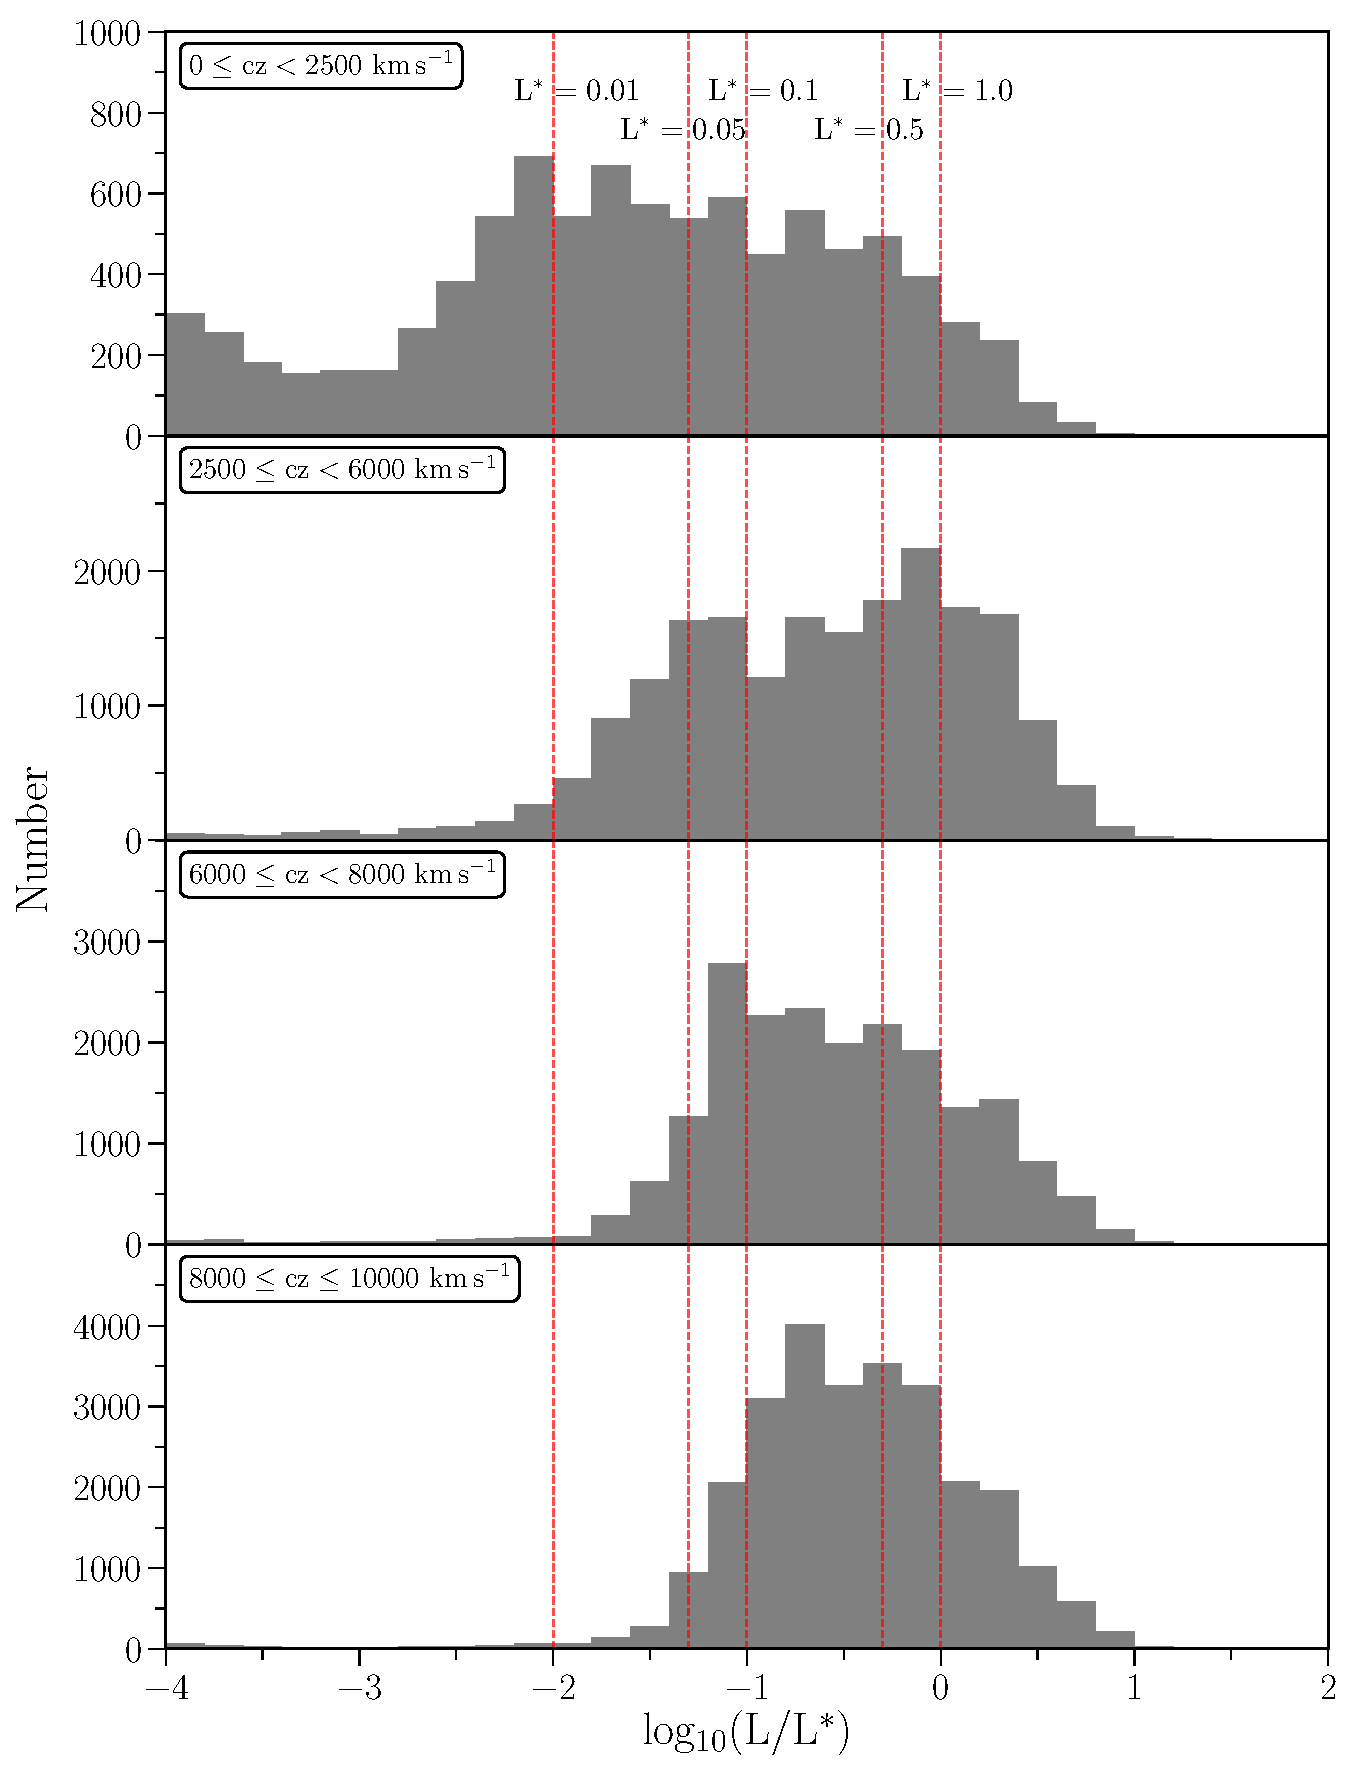
\includegraphics[width=0.8\textwidth]{Chap2/figures/Lstar_histogram_4bins_final_0-10000_v3_vert_flag0.pdf}
        \caption{\small{Distribution of $L/$\Lstar values  for all galaxies in the dataset. Red-dashed vertical lines highlight 1, 0.5, 0.1, 0.05 and 0.01 \Lstar. The turnoff in the distribution for each region reveals the corresponding completeness. We are highly complete to 0.01\Lstar out to 2500 \kms~, 0.05\Lstar between $2500 \leq cz \leq 5000$ \kms, 0.1\Lstar between $6000 \leq cz \leq 8000$ \kms, and 0.3\Lstar $8000 \leq cz \leq 10000$ \kms. See \S \ref{completeness} for a discussion of these limits.}}
        \vspace{5pt}
        \label{completeness_plot}
\end{figure} 

\begin{figure}[ht!]
        \centering
        \vspace{0pt}
        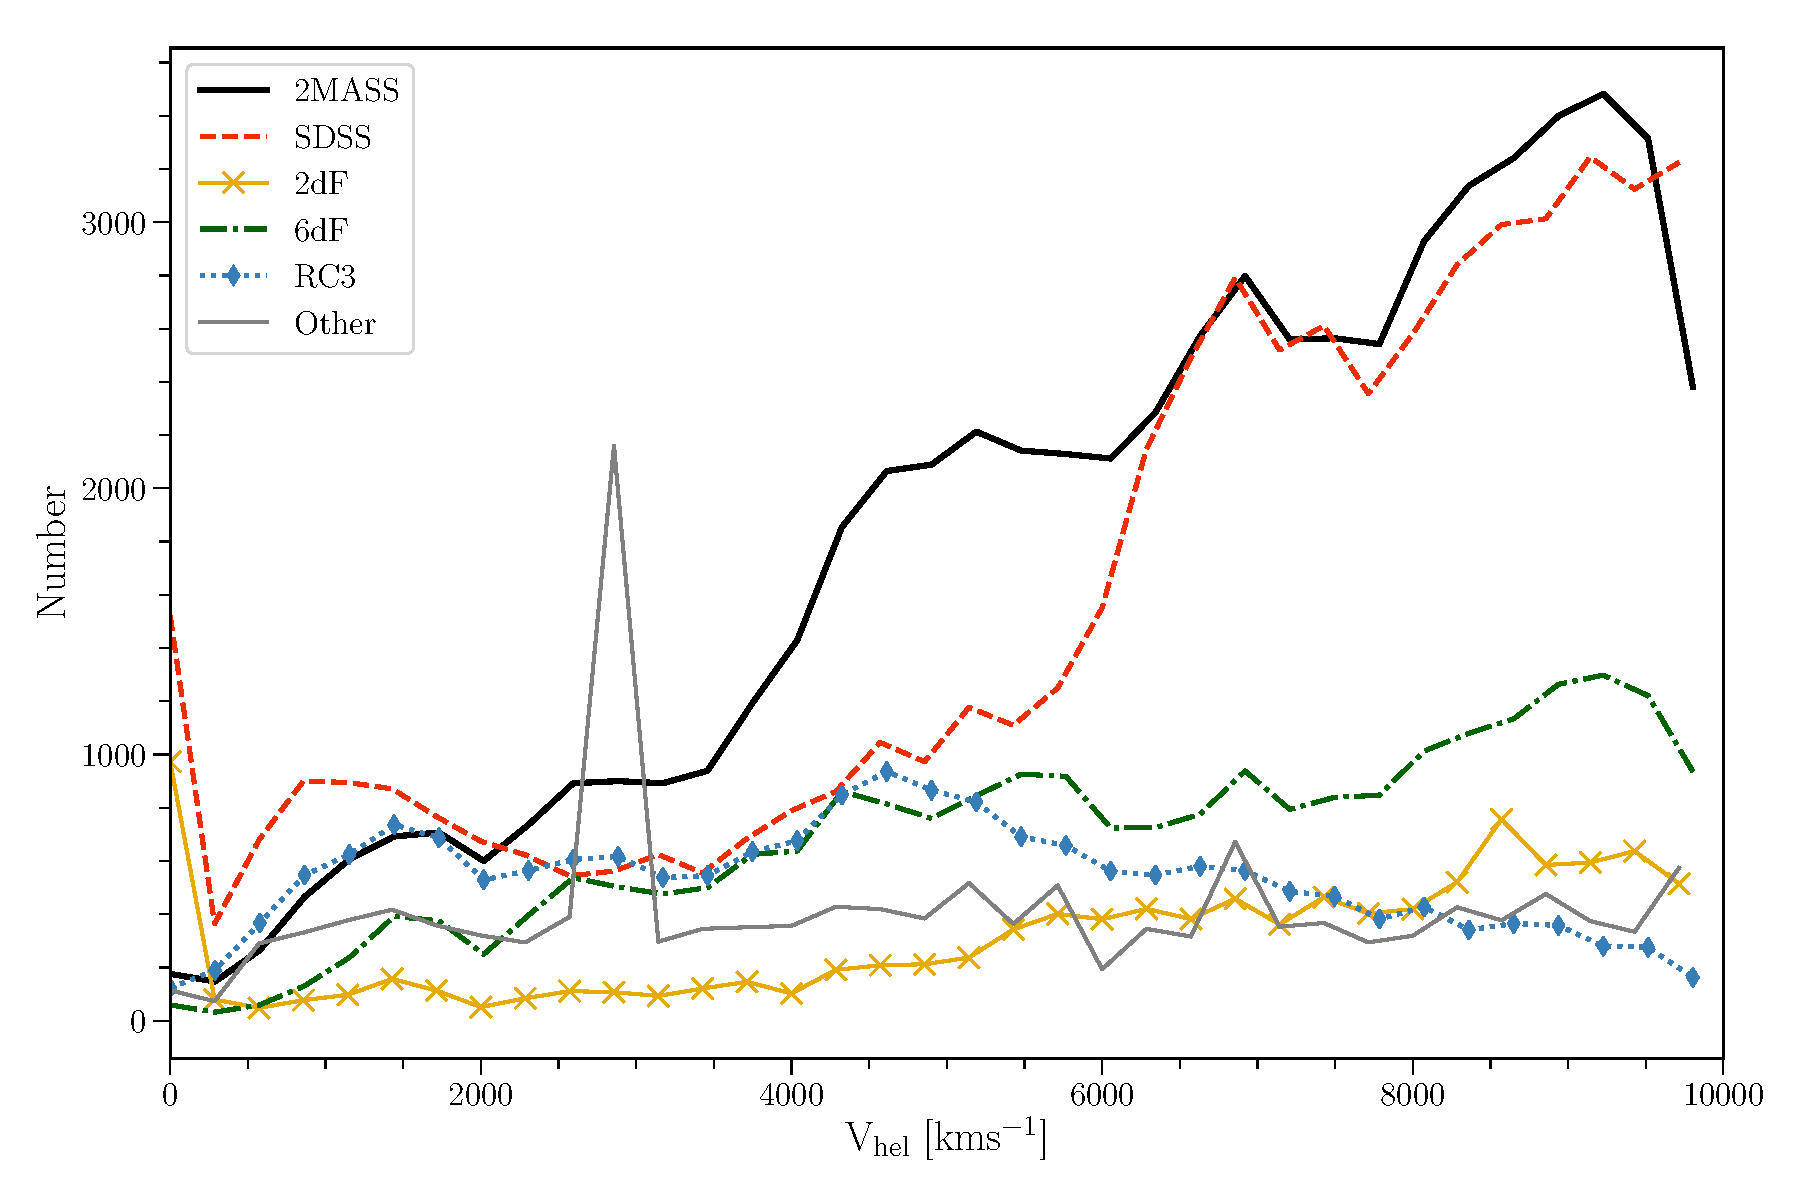
\includegraphics[width=0.99\textwidth]{Chap2/figures/hist_by_survey8_filtered_0only.pdf}
        \caption{\small{Number of objects included from the major sources 2MASS (solid-black), SDSS (dashed-red), 2dF (solid-gold-crosses), 6dF (dot-dashed-green), RC3 (dotted-diamond-blue) and all other sources (solid-grey) plotted as a function of heliocentric velocity. The peak for ``other sources" between $2500 \lesssim v_{\rm hel} \lesssim 3100$ \kms~is due to the small (1.3 square degrees) ultra-deep Suburu/XMM-Newton Deep Sky Survey (SXDS), which reaches a $B$-band magnitude limit of $B=28.2$.}}
        \vspace{5pt}
        \label{source_histograms}
\end{figure} 


%\begin{figure}[htb]
%        \centering
%        \vspace{0pt}
%        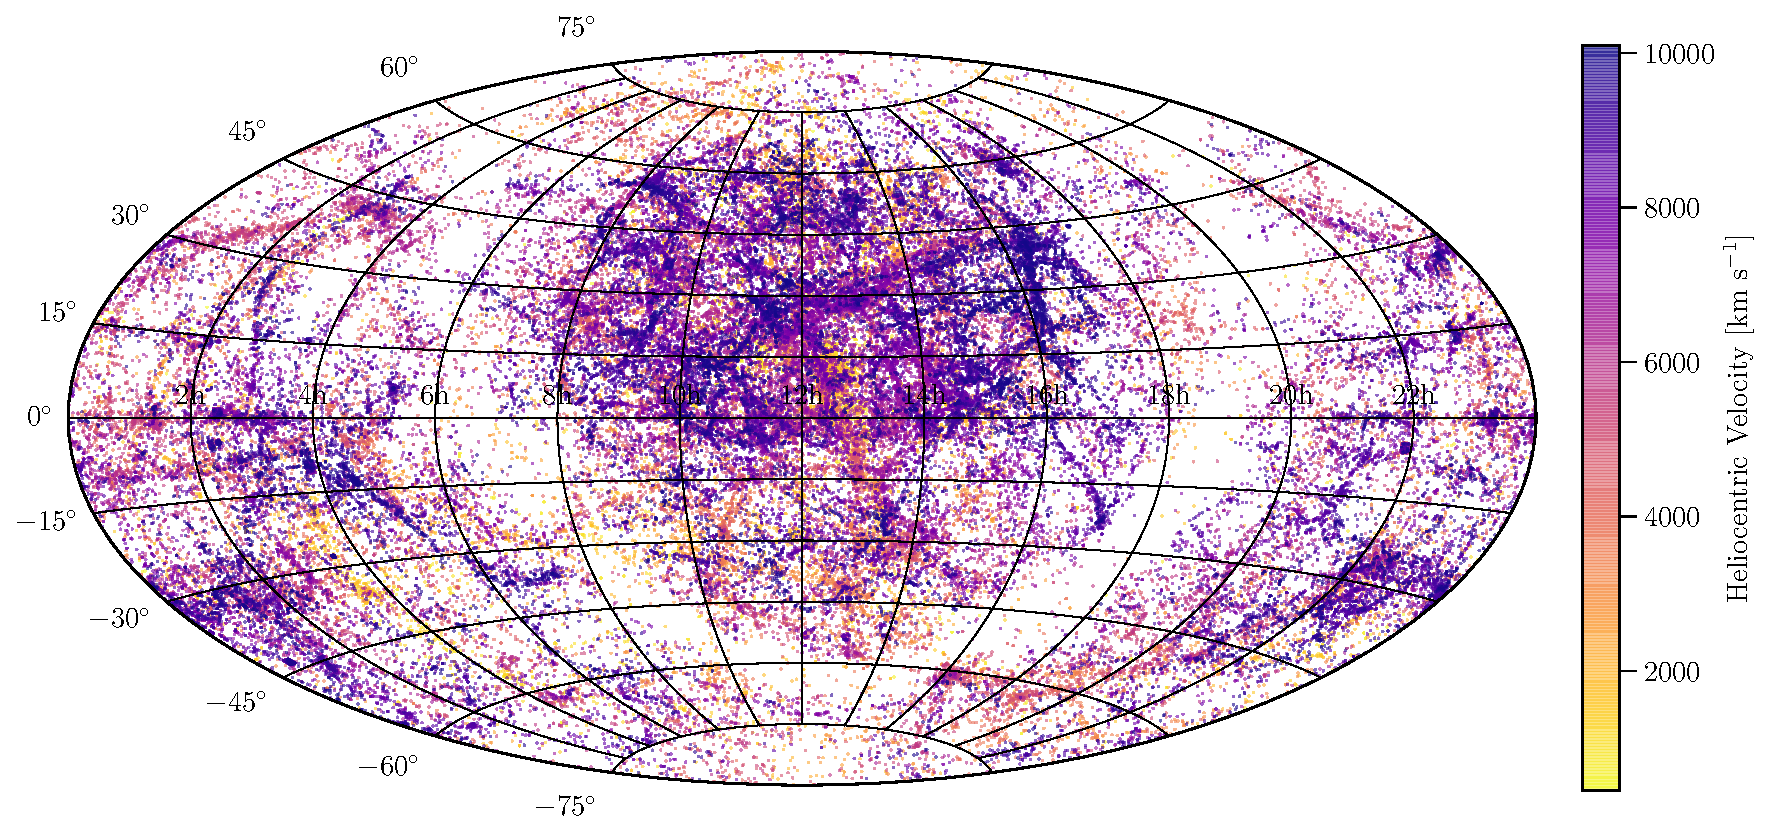
\includegraphics[width=0.999\textwidth, angle=90]{Chap2/figures/all_sky.pdf} \label{a}
%        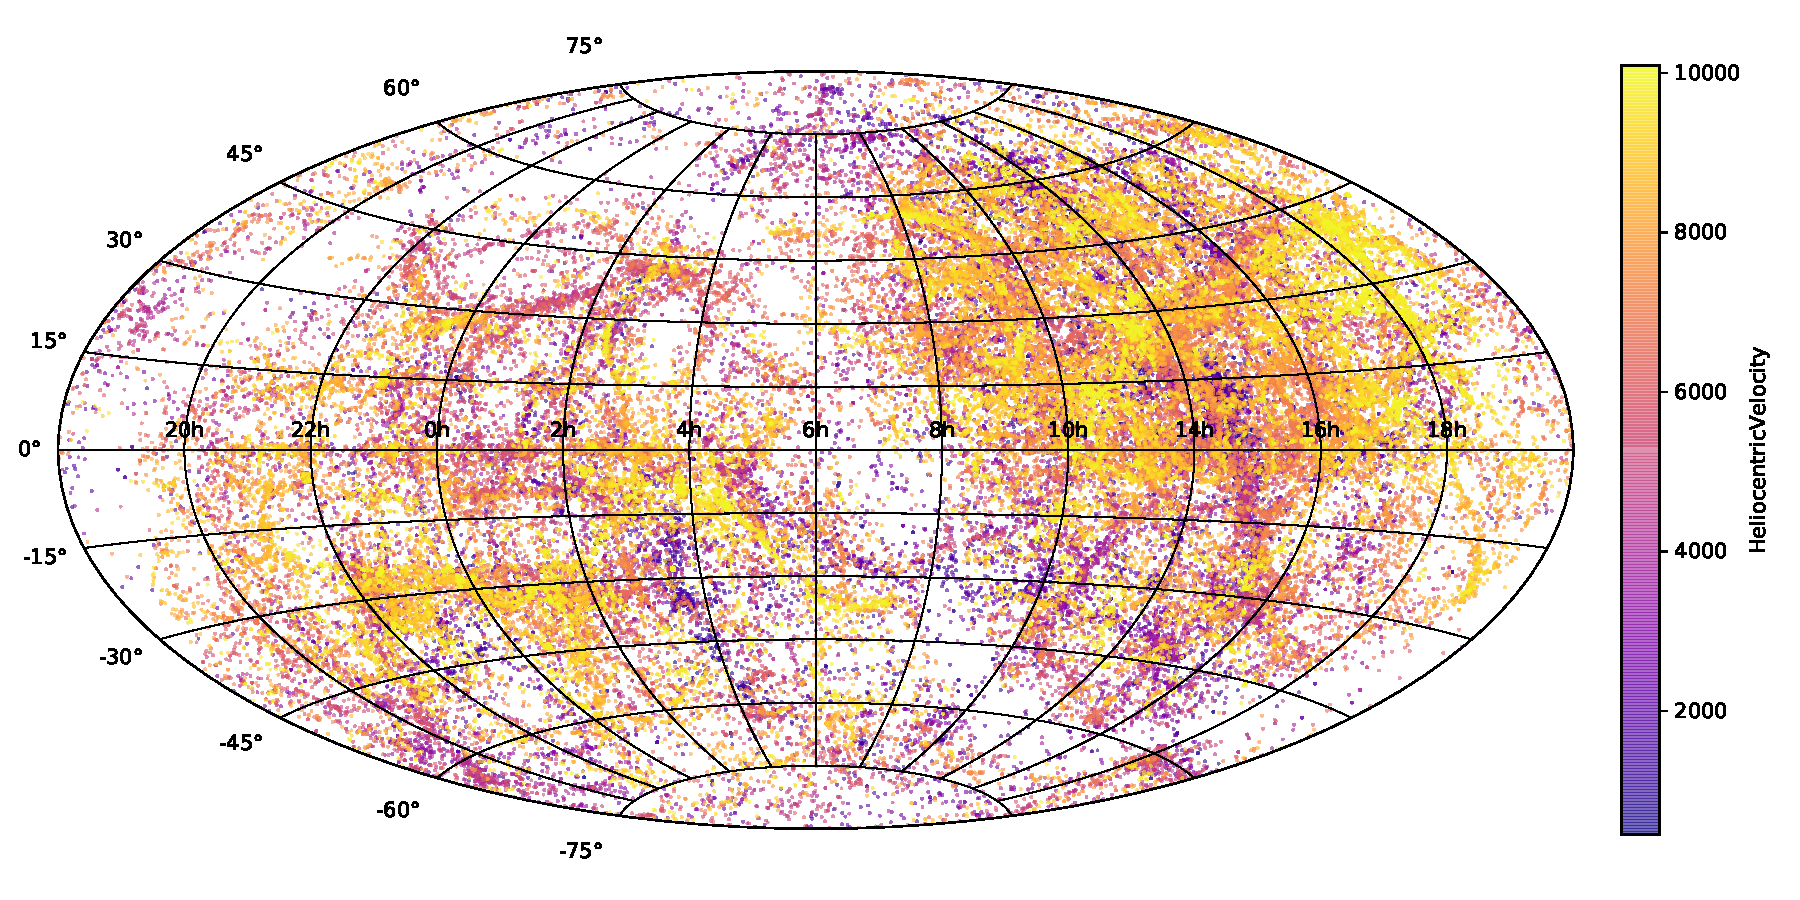
\includegraphics[width=0.99\textwidth, angle=90]{Chap2/figures/all_sky_6h.pdf} \label{b}
%        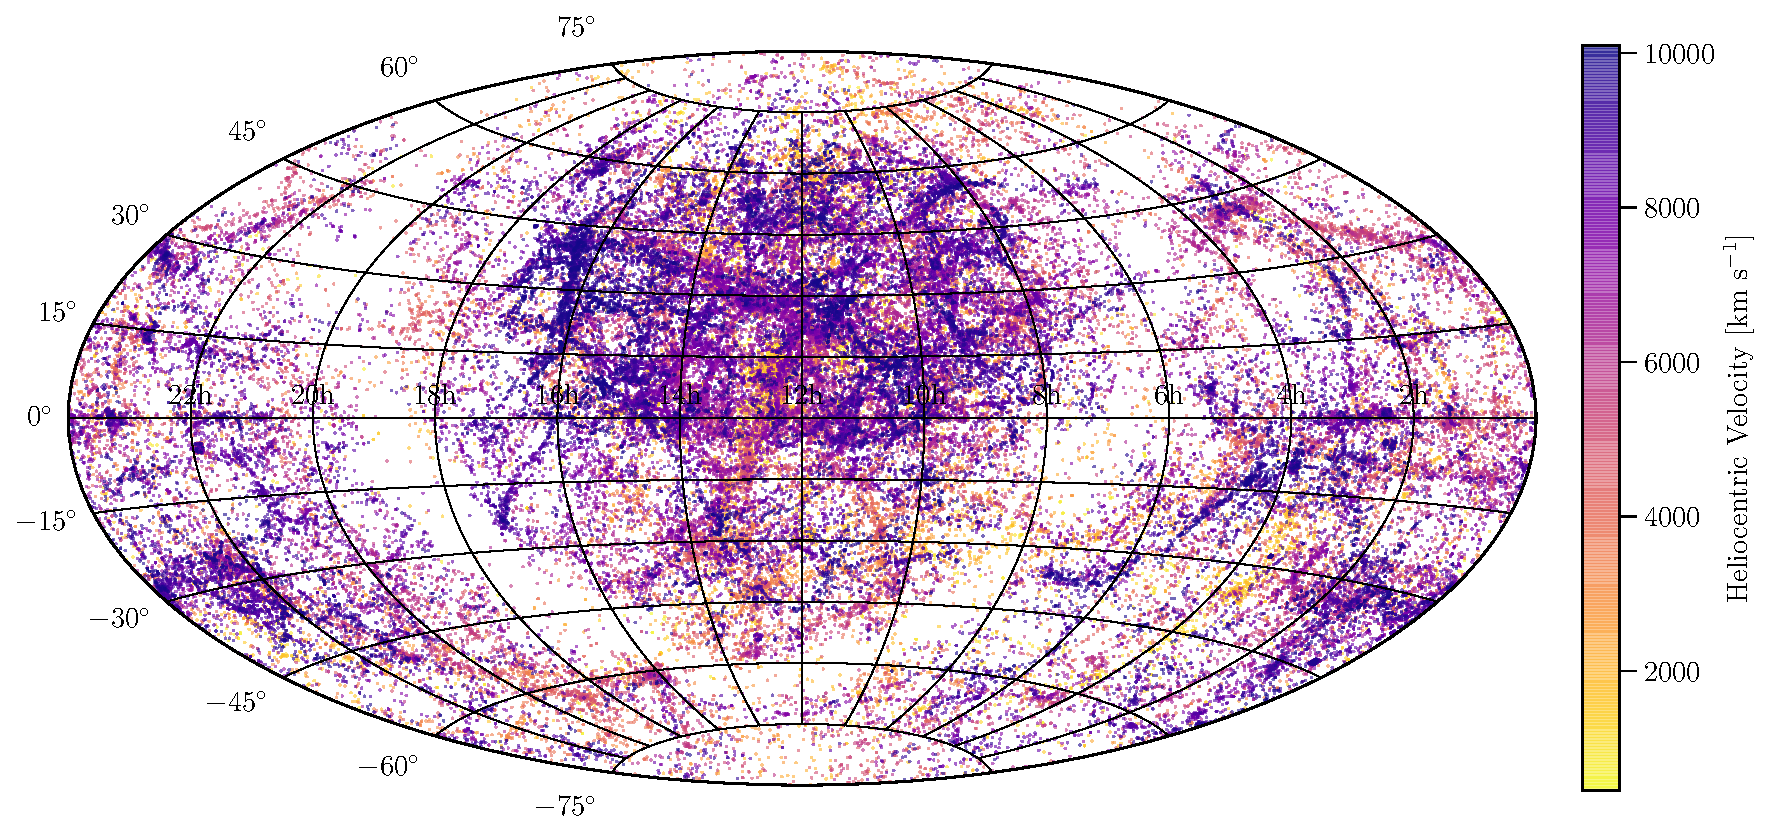
\includegraphics[width=0.99\textwidth, angle=90]{Chap2/figures/all_sky_12h.pdf} \label{c}
%        \caption{\small{The positions of all galaxies with $flag=0$ (see \ref{flag} below) plotted in Aitoff projection and colored according to heliocentric velocity. We include 3 maps, centered at \textbf{Top:} R.A. = 0h, \textbf{Center:} R.A. = 6h, and \textbf{Bottom:} R.A. = 12h. }}
%%        \vspace{5pt}
%        \label{allskyvhel}
%\end{figure}


\begin{figure}[htb!]
        \centering
        \vspace{0pt}
        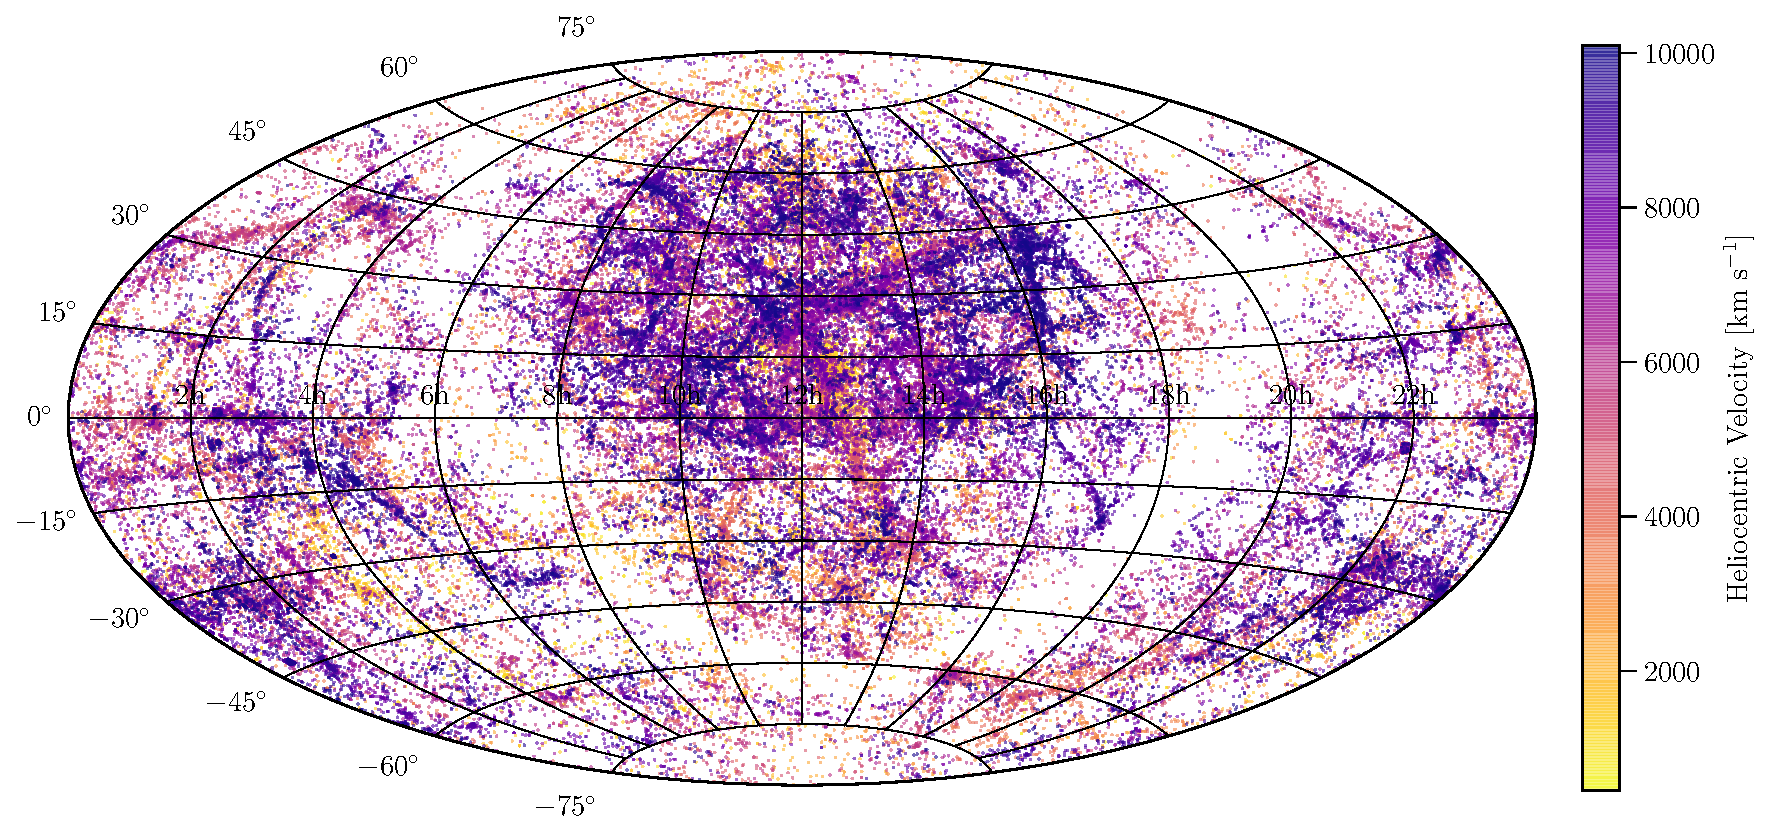
\includegraphics[width=0.55\textwidth, angle=0]{Chap2/figures/all_sky.pdf} \label{a}
        \caption{\small{The positions of all galaxies with $flag=0$ (see \ref{flag} below) plotted in Aitoff projection and colored according to heliocentric velocity. We include 3 maps, centered here at R.A. = 0h. See below for R.A. = 6h and R.A. = 12h centered maps.}}
%        \vspace{5pt}
        \label{allskyvhel}
\end{figure}
\begin{figure}[htb!]\ContinuedFloat
        \centering
        \vspace{0pt}      
        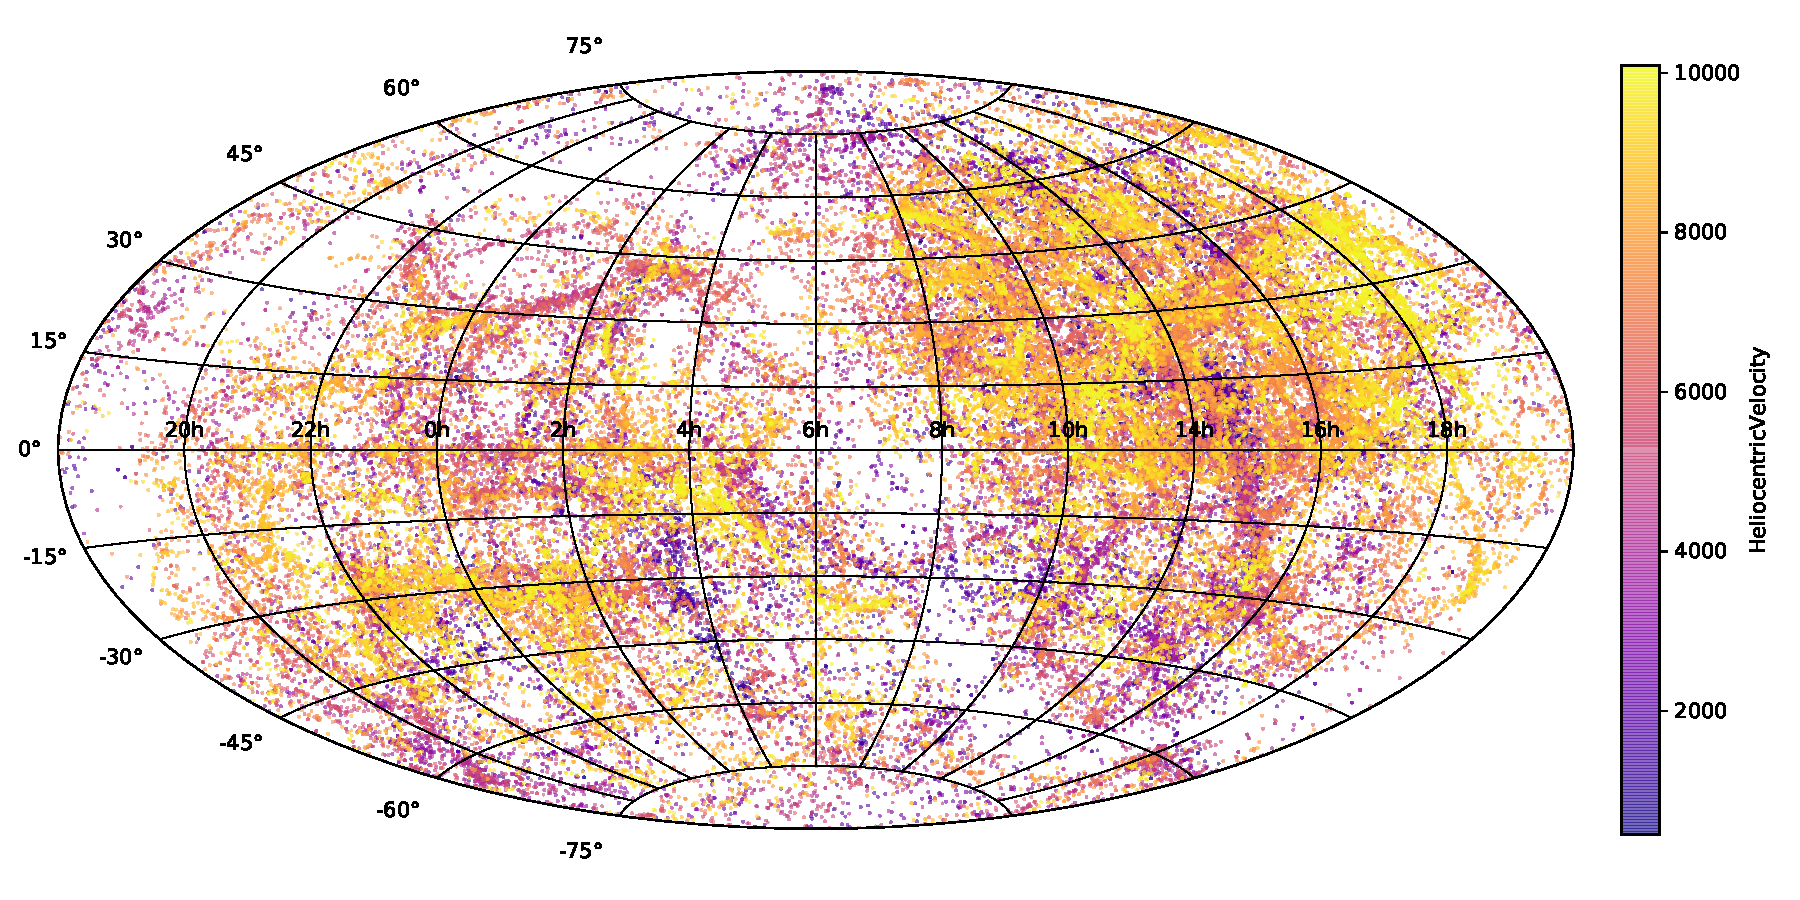
\includegraphics[width=0.55\textwidth, angle=0]{Chap2/figures/all_sky_6h.pdf} \label{b}
        \caption{\small{The positions of all galaxies with $flag=0$ (see \ref{flag} below) plotted in Aitoff projection and colored according to heliocentric velocity. We include 3 maps, centered here at R.A. = 6h. See above and below for R.A. = 0h and R.A. = 12h centered maps.}}
%        \vspace{5pt}
        \label{allskyvhel}
\end{figure}
\begin{figure}[htb!]\ContinuedFloat
        \centering
        \vspace{0pt}
        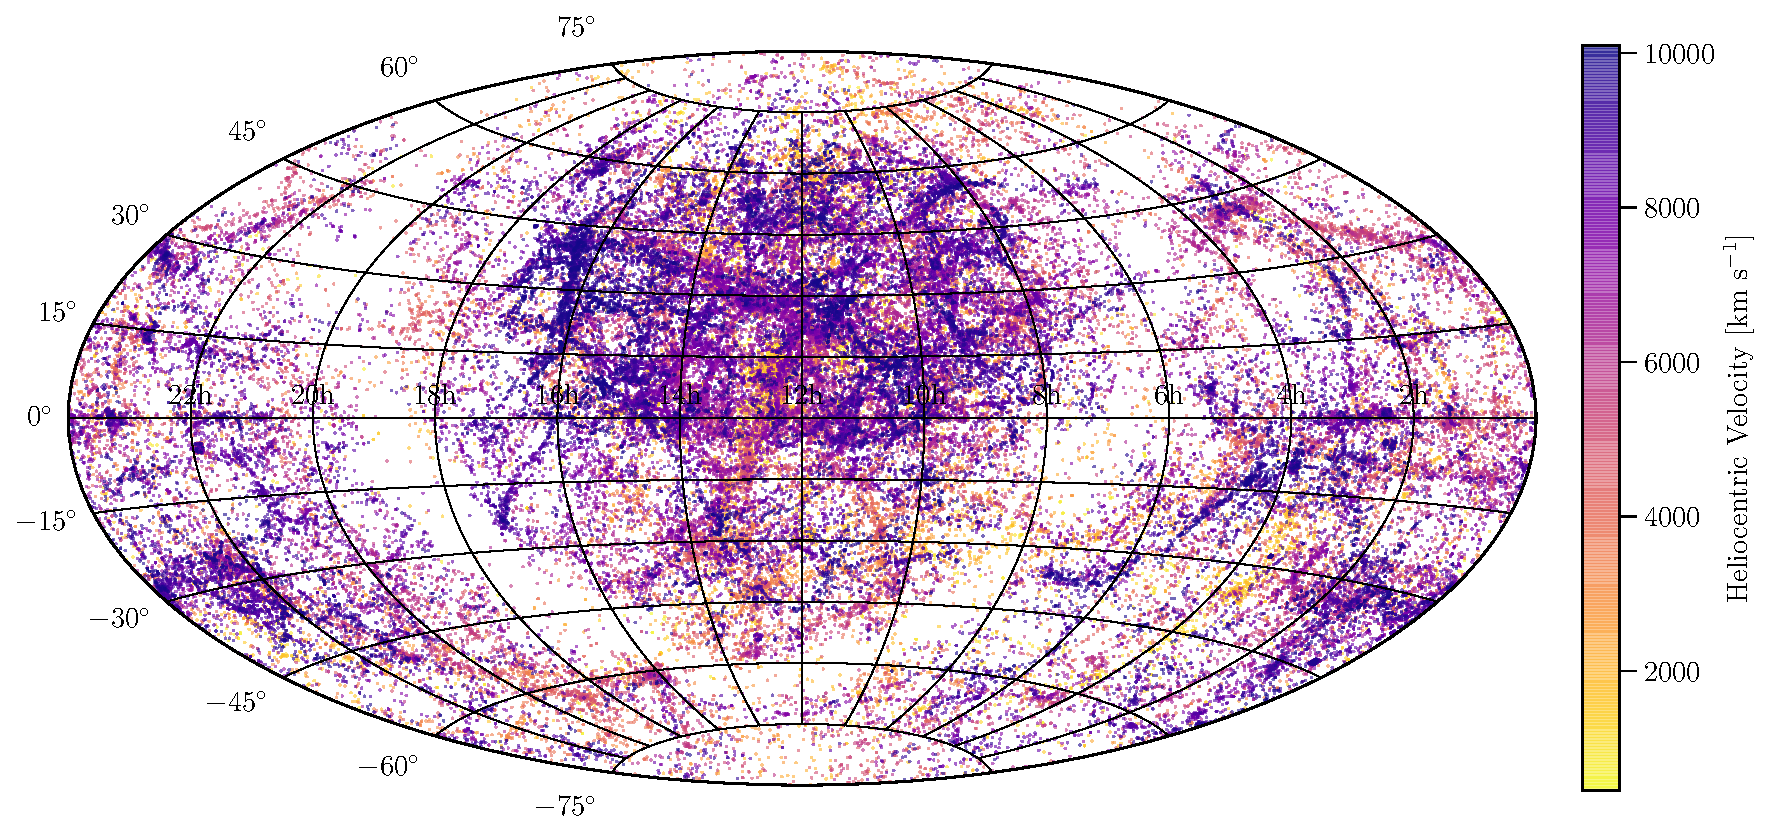
\includegraphics[width=0.55\textwidth, angle=0]{Chap2/figures/all_sky_12h.pdf} \label{c}
        \caption{\small{The positions of all galaxies with $flag=0$ (see \ref{flag} below) plotted in Aitoff projection and colored according to heliocentric velocity. We include 3 maps, centered here at R.A. = 12h. See above for R.A. = 0h and R.A. = 6h centered maps.}}
%        \vspace{5pt}
        \label{allskyvhel}
\end{figure}



The galaxy dataset contains 130,819  objects, and includes data from SDSS, 2MASS, 2dF, 6dF, RC3, and many other, smaller surveys. Figure \ref{completeness_plot} shows the number of objects as a function of luminosity in four bins of heliocentric velocity, and Figure \ref{source_histograms} shows the number of objects coming from each of the major included surveys as a function of heliocentric velocity.\footnote{The peak for ``other sources" between $2500 \lesssim v_{\rm hel} \lesssim 3100$ \kms~in Figure \ref{source_histograms} is due to the small (1.3 square degrees) ultra-deep Suburu/XMM-Newton Deep Sky Survey (SXDS), which reaches a $B$-band magnitude limit of $B=28.2$. See https://www.naoj.org/Science/SubaruProject/SXDS/} Our restricted velocity range of $cz \leq 10,000$ \kms~leads to a completeness limit of $B \lesssim 18.7$ mag, or $\sim0.2$\Lstar, at $cz = 10,000$ \kms, and progressively better towards lower velocities (see Figure \ref{completeness_plot}). This limit will vary depending on which major surveys include a particular region of the sky. The major contributor is whether or not SDSS data is available, which begins around $cz = 5,000$ \kms. Figure \ref{completeness_plot} is split into 4 velocity bins to illustrate this. Our data has a high degree of completeness down to $\sim0.01$\Lstar in the first bin, $0 \leq cz \leq 2,500$ \kms. At slightly higher velocity, $2500 \leq cz \leq 6000$ \kms, the completeness falls a bit, but is still rather complete to $\sim0.05$\Lstar as we move past the near and well studied galaxies, but have yet to reach the footprint of deep all sky surveys. SDSS data becomes available in the last two bins, spanning $6000 \leq cz \leq 10,000$ \kms, and correspondingly completeness remains high down to the SDSS limits of $B \lesssim 18.7$ mag, or $\sim0.2$\Lstar at $cz = 10,000$ \kms. 


Additionally, we note the presence of a long super-faint tail to the distribution in the low velocity bin ($0 \leq cz \leq 2,500$ \kms. This is due to a number of pointed, ultra-deep surveys which have picked up faint dwarfs in the very local universe, which then quickly exit the observability window past $v_{\rm hel} \sim 2500$ \kms~(e.g., the SXDS survey as highlighted above and in Figure \ref{source_histograms}). All luminosities are calculated as described below in \S \ref{Lstar_med}.


\section{The Catalogue}
The following section describes the contents of each column in the order it appears in the catalogue. Null values are marked in one of three ways. Columns containing strings have the null value of 'x', those containing integers have null value '-99', and those containing floating point entries have null value '-99.99'. The following subsection numbers correspond to the column numbers in the catalogue (i.e., \S \ref{Name} is the first data column, \S \ref{NEDname} is the second, etc.).

\subsection{Name} \label{Name}
Our preferred name for the galaxy. If the galaxy is in one of the following base catalogues we adopt that name, in the order of preference given below. If the galaxy is not in one of these catalogues, we use the NED-preferred name (\S \ref{NEDname}).

Name preferences: NGC, IC, UGC, UGCA, Mrk, SBS, Fairall, TOLOLO, Ton, ESO, Holm, MCG, CGCG, IRAS, IRASF, KISS, KISSR, Kaz, IZw, IIZw, IIIZw, IVZw, VZw, VIZw, VIIZw, SDSS, 3C, PG, HE, HS, PKS, FCC, FGC, HCG, VCC, KUG, PGC, 2MASS, 2dF, 6dF.

%Name preferences: NGC, IC, Mrk, UGC, UGCA, PHL, 3C, SBS, MCG, ESO, TON, TONS, PGC, PG, PB, FGC, HS, HE, KUG, IRAS, RX, CGCG, KAZ, FCC, FAIRALL, HOLM, IZw, IIZw, IIIZw, IVZw, VZw, VIZw, VIIZw, VIIIZw, IRAS, IRASF, KISS, KISSR, FBQS, LBQS, PKS, SDSS, VCC, 2MASS, 2DF, 6DF, HIPASS, 2MASX.

%NGC, MRK, UGC, PHL, 3C, IC, SBS, MCG, ISO, TON, PGC, PG, PB, FGC, HS, HE, KUG, IRAS, RX, CGCG, FBQS, LBQS, SDSS, VCC, 2MASS, 2DF, 6DF, HIPASS, 2MASX, MESSIER. 

\subsection{NEDname} \label{NEDname}
The preferred name for the galaxy in the NED database.

\subsection{z} \label{z}
The NED-preferred redshift for the galaxy. 

\subsection{RAdeg} \label{RAdeg}
Equatorial right ascension coordinate in degrees (J2000.0 epoch).

\subsection{DEdeg} \label{DEdeg}
Equatorial declination coordinate in degrees (J2000.0 epoch).

\subsection{RAh} \label{RAh}
Equatorial right ascension hour coordinate (J2000.0 epoch).

\subsection{RAm} \label{RAm}
Equatorial right ascension minute coordinate (J2000.0 epoch).

\subsection{RAs} \label{RAs}
Equatorial right ascension second coordinate (J2000.0 epoch).

\subsection{DE-} \label{DE-}
Equatorial declination coordinate sign (J2000.0 epoch).

\subsection{DEd} \label{DEd}
Equatorial declination degree coordinate (J2000.0 epoch).

\subsection{DEm} \label{DEm}
Equatorial declination minute coordinate (J2000.0 epoch).

\subsection{DEs} \label{DEs}
Equatorial declination second coordinate (J2000.0 epoch).

\subsection{GLON} \label{GLON}
Galactic longitude coordinate.

\subsection{GLAT} \label{GLAT}
Galactic latitude coordinate.

\subsection{Vhel} \label{Vhel}
Heliocentric radial velocity in \kms~units. As done by NED, we do not make any relativistic correction to these velocities.

\subsection{vcorr} \label{vcorr}
Virgocentric flow-corrected velocity. Following \cite{huchra1982, geller1983}, this is calculated as
\begin{gather*}
	vcorr = v_{\rm hel} + 300*[\sin(decl) \sin(12^{\circ}.9333) \\
	+ \\
	\cos(decl) \cos(12^{\circ}.9333) \cos(R.A. - 186^{\circ}.7833)],
\end{gather*}

\noindent which corresponds to a velocity of 300 \kms~ toward $R.A. = 186^{\circ}.7833$, $decl. = 12^{\circ}.9333$.

%\begin{eqnarray}
%\begin{centering}
%	\nonumber
%	vcorr = v_{\rm hel} + 300*[\sin(decl) \sin(12^{\circ}.9333) \\
%	\nonumber
%	+ \\
%	\cos(decl) \cos(12^{\circ}.9333) \cos(R.A. - 186^{\circ}.7833)]
%\end{centering}
%\end{eqnarray}


\subsection{distvcorr} \label{distvcorr}
Distance calculated from $vcorr$ with a Hubble constant of $H_0 = 71$ \kms $~\rm Mpc^{-1}$.

\subsection{RID\_mean} \label{RID_mean}
Mean redshift-independent distance from the NED-D catalogue \citep{tully2009}. This is the arithmetic mean of the available measurements and therefore does not correspond to any single measurement in particular.

\subsection{RID\_median} \label{RID_median}
Median redshift-independent distance from the NED-D catalogue. This is not the arithmetic median of the set, but rather the published distance value \emph{closest} to the median. The method used for this distance estimate is given by \emph{distIndicator} (\S \ref{distIndicator}).

\subsection{RID\_std} \label{RID_std}
Standard deviation of all redshift-independent distance measurements.

\subsection{RID\_min} \label{RID_min}
Minimum published redshift-independent distance.

\subsection{RID\_max} \label{RID_max}
Maximum published redshift-independent distance.

\subsection{bestDist} \label{bestDist}
Our chosen best distance estimate. This is equal to $RID\_median$ when a redshift-independent distance is available, and otherwise defaults to $distvcorr$. A redshift-independent distance estimate is available for 17,361 objects, which corresponds to 13.3\% of all objects in the catalogue. For these objects $bestDist$ is set to the median of all available redshift-independent distance estimates, and $e\_bestDist$ (\S \ref{e_bestDist}) is set to the standard deviation of all available measurements (\S \ref{RID_std}). If no error is available, $e\_bestDist$ is instead set to the standard deviation of all available redshift-independent distance measurements. When only a redshift is available, we set $bestDist$ equal to $distvcorr$ (\S \ref{distvcorr}), which is the the Hubble law distance as calculated with $H_{\rm 0} = 71$ \kms~$\rm Mpc^{-1}$ and a Virgocentric flow-corrected velocity ($vcorr$; \S \ref{vcorr}). The associated error, $e\_bestDist$, is then set to 10\% of the resulting distance estimate. At very low redshift, the uncertainty in this estimate is dominated by deviations from the Hubble Flow due to, e.g., the Local Group, and at larger distances the uncertainty in $H_{\rm 0}$ becomes dominant. The distance error for any particular galaxy is difficult to ascertain, but a 10\% error should contain the true $1\sigma$ error across our full redshift range. All galaxies with zero or negative $Vhel$ have $bestDist$ set to 1 Mpc, and $e\_bestDist$ to 0.5 Mpc (unless a redshift-independent distance is available). 

\subsection{e\_bestDist} \label{e_bestDist}
The error on $bestDist$. $e\_bestDist$ is equal to $RID\_std$ when a redshift-independent distance is available. Otherwise, $e\_bestDist$ is set to 10\% of $distvcorr$ when $vcorr \geq 0$, and 50\% of $distvcorr$ if $vcorr < 0$.


\subsection{distIndicator} \label{distIndicator}
A key indicating which method was used to measure the redshift-independent distance for this galaxy. Table \ref{distIndicators} shows the keys and their corresponding full names as compiled in the NED-D distance catalogue. This key corresponds \textit{only} to the $RID\_median$ value.


%\startlongtable
\begin{deluxetable}{llll}
\tablewidth{0pt}
\tabletypesize{\footnotesize}
\tablecaption{Distance Indicator Keys\label{distIndicators}}
\tablehead{
\colhead{Key}  	&  \colhead{Distance Indicator} 	&  \colhead{Key}	&  \colhead{Distance Indicator} }
\startdata
    AGB	&	AGB					&	MagEn    	&	Magnetic energy    	\\
    AGNtl	&	AGN time lag    		&	Mag    	&	Magnitude    	\\
    Bstar	&	B Stars				&	Maser    	&	Maser    	\\
    BCG	&	BCG					&	MassM    	&	Mass Model    	\\
    BH	&	Black Hole			&	Miras   	&	Miras    	\\
    BLLum	&	BL Lac Luminosity		&	Novae    	&	Novae    	\\
    BSG    	&	Blue Supergiant		&	OBstr    	&	OB Stars    	\\
    Brstr    	&	Brightest Stars    		&	OrMec    	&	Orbital Mech.    	\\
    Cstar    	&	Carbon Stars    			&	PAGB    	&	PAGB Stars    	\\
    Ceph    	&	Cepheids				&	PNLF    	&	PNLF    	\\
    CMD    	&	CMD					&	propM    	&	Proper Motion    	\\
    dCO    	&	CO ring diameter		&	QS    	&	Quasar spectrum    	\\
    Dsigm	&	D-Sigma				&	Radio    	&	Radio Brightness    	\\
    Scuti	&	Delta Scuti    			&	RClum    	&	Red Clump    	\\
    Diam	&	Diameter				&	DRing    	&	Ring Diameter    	\\
    dwEll	&	Dwarf Ellipticals    		&	RRLyr    	&	RR Lyrae    	\\
    Dwarf	&	Dwarf Galaxy Diameter	&	RSV    	&	RSV Stars    	\\
    EclBi	&	Eclipsing Binary		&	RV    	&	RV Stars    	\\
    FJ		&	Faber-Jackson			&	SDorS    	&	S Doradus Stars    	\\
    FGLR	&	FGLR				&	SBF    	&	SBF    	\\
    GLens	&	G Lens				&	SGRB    	&	SGRB    	\\
    GCFP	&	GC FP				&	SNIa    	&	SNIa    	\\
    GCKJK	&	GC K vs. (J-K)			&	SNIIo    	&	SNII optical    	\\
    GCrad	&	GC radius				&	SNIIr    	&	SNII radio    	\\
    GCLF	&	GCLF				&	SNIas    	&	SNIa SDSS    	\\
    GCSBF	&	GC SBF				&	Stat    	&	Statistical    	\\
    gamma	&	GeV TeV ratio			&	Sosie    	&	Sosies    	\\
    GSGD	&	Grav. Stability Gas. Disk 	&	subDw    	&	Subdwarf fitting    	\\
    GRB	&	GRB					&	SXPS	&	SX Phe Stars    	\\
    HIod	&	H I + optical distribution	&	SZ    	&	SZ effect    	\\
    HIILF	&	HII LF				&	Terti		&	Tertiary    	\\
    dHII	&	HII region diameter		&	TRGB    	&	TRGB    	\\
    HB	&	Horizontal Branch    		&	TFest    	&	Tully est    	\\
    IRAS	&	IRAS    				&	TF		&	Tully-Fisher    	\\
    Jet	&	Jet Proper Motion    		&	CepII    	&	Type II Cepheids    	\\
    LHbs	&	L(H $\beta$)-$\sigma$	&	WD    	&	White Dwarfs    	\\
    LSB	&	LSB galaxies			&	WR    	&	Wolf-Rayet    	\\
    Mstar	&	M Stars				&			&				\\
\enddata 
\tablecomments{Distance indicators and associated keys. Full descriptions can be found at \url{https://ned.ipac.caltech.edu/Library/Distances/distintro.html}}
\vspace{-5pt}
\end{deluxetable}


%\begin{center}
%\begin{longtable}{llll}
%  \caption[Short caption]{Long captions for the long table.} \label{tab:long1} \\
%  % First head
%  \hline
%  % The table
%    AGB	&	AGB					&	MagEn    	&	Magnetic energy    	\\
%    AGNtl	&	AGN time lag    		&	Mag    	&	Magnitude    	\\
%    Bstar	&	B Stars				&	Maser    	&	Maser    	\\
%    BCG	&	BCG					&	MassM    	&	Mass Model    	\\
%    BH	&	Black Hole			&	Miras   	&	Miras    	\\
%    BLLum	&	BL Lac Luminosity		&	Novae    	&	Novae    	\\
%    BSG    	&	Blue Supergiant		&	OBstr    	&	OB Stars    	\\
%    Brstr    	&	Brightest Stars    		&	OrMec    	&	Orbital Mech.    	\\
%    Cstar    	&	Carbon Stars    			&	PAGB    	&	PAGB Stars    	\\
%    Ceph    	&	Cepheids				&	PNLF    	&	PNLF    	\\
%    CMD    	&	CMD					&	propM    	&	Proper Motion    	\\
%    dCO    	&	CO ring diameter		&	QS    	&	Quasar spectrum    	\\
%    Dsigm	&	D-Sigma				&	Radio    	&	Radio Brightness    	\\
%    Scuti	&	Delta Scuti    			&	RClum    	&	Red Clump    	\\
%    Diam	&	Diameter				&	DRing    	&	Ring Diameter    	\\
%    dwEll	&	Dwarf Ellipticals    		&	RRLyr    	&	RR Lyrae    	\\
%    Dwarf	&	Dwarf Galaxy Diameter	&	RSV    	&	RSV Stars    	\\
%    EclBi	&	Eclipsing Binary		&	RV    	&	RV Stars    	\\
%    FJ		&	Faber-Jackson			&	SDorS    	&	S Doradus Stars    	\\
%    FGLR	&	FGLR				&	SBF    	&	SBF    	\\
%    GLens	&	G Lens				&	SGRB    	&	SGRB    	\\
%    GCFP	&	GC FP				&	SNIa    	&	SNIa    	\\
%    GCKJK	&	GC K vs. (J-K)			&	SNIIo    	&	SNII optical    	\\
%    GCrad	&	GC radius				&	SNIIr    	&	SNII radio    	\\
%    GCLF	&	GCLF				&	SNIas    	&	SNIa SDSS    	\\
%    GCSBF	&	GC SBF				&	Stat    	&	Statistical    	\\
%    gamma	&	GeV TeV ratio			&	Sosie    	&	Sosies    	\\
%    GSGD	&	Grav. Stability Gas. Disk 	&	subDw    	&	Subdwarf fitting    	\\
%    GRB	&	GRB					&	SXPS	&	SX Phe Stars    	\\
%    HIod	&	H I + optical distribution	&	SZ    	&	SZ effect    	\\
%    HIILF	&	HII LF				&	Terti		&	Tertiary    	\\
%    dHII	&	HII region diameter		&	TRGB    	&	TRGB    	\\
%    HB	&	Horizontal Branch    		&	TFest    	&	Tully est    	\\
%    IRAS	&	IRAS    				&	TF		&	Tully-Fisher    	\\
%    Jet	&	Jet Proper Motion    		&	CepII    	&	Type II Cepheids    	\\
%    LHbs	&	L(H $\beta$)-$\sigma$	&	WD    	&	White Dwarfs    	\\
%    LSB	&	LSB galaxies			&	WR    	&	Wolf-Rayet    	\\
%    Mstar	&	M Stars				&			&				\\
%\end{longtable}
%\end{center}




%\begin{center}
%\begin{longtable}{llll}
%%Here is the caption, the stuff in [] is the table of contents entry,
%%the stuff in {} is the title that will appear on the first page of the
%%table.
%\caption[Distance Indicator Keys]{Distance Indicator Keys} \label{distIndicators} \\
%
%%This is the header for the first page of the table...
%\hline \hline \\[-2ex]
%   \multicolumn{1}{c}{Key} &
%   \multicolumn{1}{c}{Distance Indicator} &
%   \multicolumn{1}{c}{Key} &
%   \multicolumn{1}{c}{Distance Indicator} \\[0.5ex] \hline
%   \\[-1.8ex]
%\endfirsthead
%
%%This is the header for the remaining page(s) of the table...
%\multicolumn{4}{c}{{\tablename} \thetable{} -- Continued} \\[0.5ex]
%  \hline \hline \\[-2ex]
%   \multicolumn{1}{c}{Key} &
%   \multicolumn{1}{c}{Distance Indicator} &
%   \multicolumn{1}{c}{Key} &
%   \multicolumn{1}{c}{Distance Indicator} \\[0.5ex] \hline
%  \\[-1.8ex]
%\endhead
%
%%This is the footer for all pages except the last page of the table...
%  \multicolumn{4}{l}{{Continued on Next Page\ldots}} \\
%\endfoot
%
%%This is the footer for the last page of the table...
%  \\[-1.8ex] \hline \hline
%\endlastfoot
%
%%Now the data...
%    AGB	&	AGB					&	MagEn    	&	Magnetic energy    	\\
%    AGNtl	&	AGN time lag    		&	Mag    	&	Magnitude    	\\
%    Bstar	&	B Stars				&	Maser    	&	Maser    	\\
%    BCG	&	BCG					&	MassM    	&	Mass Model    	\\
%    BH	&	Black Hole			&	Miras   	&	Miras    	\\
%    BLLum	&	BL Lac Luminosity		&	Novae    	&	Novae    	\\
%    BSG    	&	Blue Supergiant		&	OBstr    	&	OB Stars    	\\
%    Brstr    	&	Brightest Stars    		&	OrMec    	&	Orbital Mech.    	\\
%    Cstar    	&	Carbon Stars    			&	PAGB    	&	PAGB Stars    	\\
%    Ceph    	&	Cepheids				&	PNLF    	&	PNLF    	\\
%    CMD    	&	CMD					&	propM    	&	Proper Motion    	\\
%    dCO    	&	CO ring diameter		&	QS    	&	Quasar spectrum    	\\
%    Dsigm	&	D-Sigma				&	Radio    	&	Radio Brightness    	\\
%    Scuti	&	Delta Scuti    			&	RClum    	&	Red Clump    	\\
%    Diam	&	Diameter				&	DRing    	&	Ring Diameter    	\\
%    dwEll	&	Dwarf Ellipticals    		&	RRLyr    	&	RR Lyrae    	\\
%    Dwarf	&	Dwarf Galaxy Diameter	&	RSV    	&	RSV Stars    	\\
%    EclBi	&	Eclipsing Binary		&	RV    	&	RV Stars    	\\
%    FJ		&	Faber-Jackson			&	SDorS    	&	S Doradus Stars    	\\
%    FGLR	&	FGLR				&	SBF    	&	SBF    	\\
%    GLens	&	G Lens				&	SGRB    	&	SGRB    	\\
%    GCFP	&	GC FP				&	SNIa    	&	SNIa    	\\
%    GCKJK	&	GC K vs. (J-K)			&	SNIIo    	&	SNII optical    	\\
%    GCrad	&	GC radius				&	SNIIr    	&	SNII radio    	\\
%    GCLF	&	GCLF				&	SNIas    	&	SNIa SDSS    	\\
%    GCSBF	&	GC SBF				&	Stat    	&	Statistical    	\\
%    gamma	&	GeV TeV ratio			&	Sosie    	&	Sosies    	\\
%    GSGD	&	Grav. Stability Gas. Disk 	&	subDw    	&	Subdwarf fitting    	\\
%    GRB	&	GRB					&	SXPS	&	SX Phe Stars    	\\
%    HIod	&	H I + optical distribution	&	SZ    	&	SZ effect    	\\
%    HIILF	&	HII LF				&	Terti		&	Tertiary    	\\
%    dHII	&	HII region diameter		&	TRGB    	&	TRGB    	\\
%    HB	&	Horizontal Branch    		&	TFest    	&	Tully est    	\\
%    IRAS	&	IRAS    				&	TF		&	Tully-Fisher    	\\
%    Jet	&	Jet Proper Motion    		&	CepII    	&	Type II Cepheids    	\\
%    LHbs	&	L(H $\beta$)-$\sigma$	&	WD    	&	White Dwarfs    	\\
%    LSB	&	LSB galaxies			&	WR    	&	Wolf-Rayet    	\\
%    Mstar	&	M Stars				&			&				\\
%\tablecomments{Distance indicators and associated keys. Full descriptions can be found at \url{https://ned.ipac.caltech.edu/Library/Distances/distintro.html}}
%\end{longtable}
%\end{center}





\subsection{MajDiam\_ang} \label{diameters}
Major axis diameter in units of arcsec. We have homogenized the galaxy data beyond the steps taken by NED by normalizing diameter measurements to 2MASS $K$-band values. Most galaxies in NED have measures of inclination, position angle and diameter available in several different bands, so in order to make more meaningful comparisons we choose one band for all measurements. We chose 2MASS values for this because it is an all-sky survey, and represents a large fraction of available galaxy data. Physical galaxy diameters are derived from 2MASS $K_s$ ``total" angular diameter measurements and galaxy distances. 2MASS $K_s$ ``total" diameter estimates are surface brightness extrapolation measurements and were derived by the 2MASS team as 

\begin{equation}
r_{tot} = r' + a ln(148)^b,
\end{equation}

\noindent where $r_{tot}$ is defined as the point where the surface brightness extends to 5 disk scale lengths, $r'$ is the starting point radius ($>5" - 10"$ beyond the nucleus, or core influence), and $a$ and $b$ are Sersic exponential function scale length parameters ($f = f_0 \exp{(-r/a)}^{(1/b)}$, see \citealt{jarrett2003} for a full description). Approximately $50\%$ of all the galaxies have this 2MASS $K_s$ ``total" diameter. Of the remainder, $20\%$ have SDSS diameters, $3\%$ have diameters from other surveys, and $27\%$ have no published diameter. 

For galaxies with multiple published measurements from different facilities, we have derived linear fits in order to convert between them. The orthogonal distance regression (ODR) algorithm as implemented by the Fortran code ODRPACK (and the Python wrapped version included in the Scipy package) was used to derive these best fits and their associated errors. ODR, compared to the more common linear regression algorithm, assumes errors in both x- and y-coordinates and thus minimizes the orthogonal distance between both dependent and independent data and the fit. We then ranked the available surveys in order of goodness of fit to 2MASS values. The fits for each survey are listed in Table \ref{diameter_fits}. 

A significant fraction of galaxies have irregular, incomplete, or otherwise suspect diameter data as published in NED. For example, some have 2MASS $K_s$ ``total" diameters available, but the published axis ratio (i.e., the ratio of minor to major axis) is either greater than 1, or otherwise significantly deviates from that found in other surveys. Furthermore, often our highest ranking diameter survey has incomplete data (such as a missing axis ratio or position angle measurement). For our purposes we want to choose a single, representative value for each parameter. Our method for choosing this value is as follows: 1) we choose the highest ranking diameter measurement available, and choose the largest major-axis diameter value when multiple are available from the same facility, 2) we choose the highest ranking axes ratio, preferentially selecting the value from the measurement chosen in (1), but rejecting a ratio = 1 when the average ratio of all measurements is less than 1, 3) we choose the highest ranking position angle measurement, again preferentially selecting the value included in (1).

Finally, we check to see if our initial choices are outliers using a version of the Iglewicz-Hoaglin Method, a median absolute deviation algorithm \citep{iglewicz1993}. This works by calculating the so-called ``modified z-score" for each value, $M_i$, as follows:

\begin{equation}
M_{i} = \frac{0.6745 (x_i - \tilde{x})}{MAD},
\end{equation}
\noindent where $\tilde{x}$ is the median of the dataset, and MAD is the median absolute deviation. This modified z-score is then compared to a threshold to determine if $x_i$ is an outlier or not. Through trial-and-error we set our outlier thresholds at 14.0 for major axis diameters, 3.5 for position angles, and 2.0 for axis ratios. Smaller threshold values indicate a stricter outlier rejection. If our initial choice of any of these values is flagged as an outlier, we choose the next highest-ranking, non-outlier value. The decision of diameter, ratio and position angle for each galaxy is included in the $diameter\_key$ (\ref{diameter_key}), $ratio\_key$ (\ref{ratio_key}), and $pa\_key$ (\ref{pa_key}) columns. In Figure \ref{magvdiam} we show the relationship between our resulting galaxy diameters and median absolute magnitudes (calculated with $Bmag$ and $bestDist$, see below), along with a best fit line in blue and the \cite{wakker2009} fit shown in red for comparison.


%Finally, we also compute an estimate of the virial radius of each galaxy as $log R_{vir} = 0.69 log D + 1.24$. This follows the parametrization of Stocke et al. (2013) relating a galaxy's luminosity to its virial radius, and the Wakker $\&$ Savage (2009) empirical relation between diameter and luminosity (see Wakker et al. 2015 and references therein for further details). Errors are propagated from the original published magnitude errors.



\begin{deluxetable}{l c c c c c c}
\tablewidth{0pt}
\setlength{\tabcolsep}{0.04in} 
\tabletypesize{\footnotesize}
\rotate
\tablecaption{Summary of Diameter, Ratio, and P.A. Sources and Fits\label{diameter_fits}}
\tablehead{
\colhead{Source of Data}  			&  \colhead{Table Key} &  \colhead{m}  		&  \colhead{b}			& \colhead{Diameter Total} &  \colhead{Ratio Total} &  \colhead{P.A. Total}}
%\colnumbers
\startdata
K\_s (2MASS ``Total")			& K\_2mass\_tot	& $N/A$				& $N/A$				&	62945		& 53778		& 57990	\\
K\_s (LGA/2MASS ``Total")		& K\_lga2mass\_tot	& $N/A$				& $N/A$				&	593			& 497		& 553	\\
K\_s (2MASS isophotal)			& K\_2mass\_iso	& $1.765 \pm 0.003$		& $1.31 \pm 0.06$		&	371			& 0			& 0		\\
POSS1 103a-O					& poss\_103a-O	& $0.87 \pm  0.01$		& $17.60 \pm 0.35$		&      3466			& 5151		& 1513	\\
POSS1 103a-E					& poss\_103a-E	& $1.05 \pm 0.04$		& $26.22 \pm 1.98$		&	121			& 341		& 1		\\
ESO-LV ``Quick Blue" IIa-O		& eso-lv			& $0.81 \pm 0.02$		& $-9.73 \pm 1.37$		&	1442			& 4858		& 3167	\\
r (SDSS Isophotal)				& r\_sdss\_iso		& $1.03 \pm 0.01$		& $0.84 \pm 0.17$		&	26802		& 19726		& 25004	\\
RC3 D\_0 (blue)				& rc3\_d0			& $1.04 \pm 0.01$		& $-1.29 \pm 0.58$		&	277			& 0			& 0		\\
RC3 D\_25, R\_25 (blue)			& rc3\_dr\_25		& $1.11 \pm 0.01$		& $-3.09 \pm 0.60$		&	1			& 278		& 139	\\
r (SDSS Petrosian)				& r\_sdss\_pet		& $4.73 \pm 0.03$		& $3.38 \pm 0.21$		&	869			& 0			& 0		\\
%r (SDSS deVaucouleurs)			& $3.49 \pm 0.04$		& $14.45 \pm 0.21$		&	XXX			\\
r (SDSS de Vaucouleurs)			& r\_sdss\_dev		& $2.70 \pm 0.04$		& $15.64 \pm 0.22$		&	51			& 12302		& 7107	\\
%RC3 A\_e (Johnson B)			& $2.25 \pm 0.06$		& $19.20 \pm 1.78$		&	XXX			\\
%r (SDSS Exponential)			& r\_sdss\_exp		& $8.24 \pm 0.06$		& $7.73 \pm 0.20$		&	0			& 0			& 0		\\
%B (Johnson)					&				& $1.24 \pm 0.09$		& $-25.31 \pm 9.73$		&	0			\\
R (Kron-Cousins)				& R\_kron\_cousins	& $1.47 \pm 0.14$		& $-35.89 \pm 14.41$	&	0			& 0			& 3		\\
ESO-Uppsala ``Quick Blue" IIa-O	& eso\_upp		& $1.06 \pm 0.02$		& $-13.39 \pm 1.38$		&	181			& 180		& 132	\\
%ESO-LV IIIa-F					& $4.65 \pm 0.13$		& $23.02 \pm 0.92$		&	XXX			\\
\enddata
%\tablenotetext{a}{Total exposure time and S/N ratio is given for multi-orbit exposures.}
\tablecomments{Diameter fits in order of preference. (1) The source name of the data given by NED. (2) The corresponding source key given in the catalogue. (3), (4) The slope and y-intercept of the ODR best fit with errors. (5), (6), (7) The total number of diameters, diameter ratios, and position angles coming from each source.}
\end{deluxetable}




%\begin{table*}[ht]\footnotesize
%\begin{center}
%\begin{tabular}{l c c c c c c}
% \hline \hline
% Survey Name                			& Table Key		& m   				& b					& Diameter Total 	& Ratio Total	& P.A. Total	\\
%  \hline \hline 
%K\_s (2MASS ``Total")			& K\_2mass\_tot	& $N/A$				& $N/A$				&	62945		& 53778		& 57990	\\
%K\_s (LGA/2MASS "total")			& K\_lga2mass\_tot	& $N/A$				& $N/A$				&	593			& 497		& 553	\\
%K\_s (2MASS isophotal)			& K\_2mass\_iso	& $1.765 \pm 0.003$		& $1.31 \pm 0.06$		&	371			& 0			& 0		\\
%POSS1 103a-O					& poss\_103a-O	& $0.87 \pm  0.01$		& $17.60 \pm 0.35$		&      3466			& 5151		& 1513	\\
%POSS1 103a-E					& poss\_103a-E	& $1.05 \pm 0.04$		& $26.22 \pm 1.98$		&	121			& 341		& 1		\\
%ESO-LV ``Quick Blue" IIa-O		& eso-lv			& $0.81 \pm 0.02$		& $-9.73 \pm 1.37$		&	1442			& 4858		& 3167	\\
%r (SDSS Isophotal)				& r\_sdss\_iso		& $1.03 \pm 0.01$		& $0.84 \pm 0.17$		&	26802		& 19726		& 25004	\\
%RC3 D\_0 (blue)				& rc3\_d0			& $1.04 \pm 0.01$		& $-1.29 \pm 0.58$		&	277			& 0			& 0		\\
%RC3 D\_25, R\_25 (blue)			& rc3\_dr\_25		& $1.11 \pm 0.01$		& $-3.09 \pm 0.60$		&	1			& 278		& 139	\\
%r (SDSS Petrosian)				& r\_sdss\_pet		& $4.73 \pm 0.03$		& $3.38 \pm 0.21$		&	869			& 0			& 0		\\
%%r (SDSS deVaucouleurs)			& $3.49 \pm 0.04$		& $14.45 \pm 0.21$		&	XXX			\\
%r (SDSS de Vaucouleurs)			& r\_sdss\_dev		& $2.70 \pm 0.04$		& $15.64 \pm 0.22$		&	51			& 12302		& 7107	\\
%%RC3 A\_e (Johnson B)			& $2.25 \pm 0.06$		& $19.20 \pm 1.78$		&	XXX			\\
%%r (SDSS Exponential)			& r\_sdss\_exp		& $8.24 \pm 0.06$		& $7.73 \pm 0.20$		&	0			& 0			& 0		\\
%%B (Johnson)					&				& $1.24 \pm 0.09$		& $-25.31 \pm 9.73$		&	0			\\
%R (Kron-Cousins)				& R\_kron\_cousins	& $1.47 \pm 0.14$		& $-35.89 \pm 14.41$	&	0			& 0			& 3		\\
%ESO-Uppsala ``Quick Blue" IIa-O	& eso\_upp		& $1.06 \pm 0.02$		& $-13.39 \pm 1.38$		&	181			& 180		& 132	\\
%%ESO-LV IIIa-F					& $4.65 \pm 0.13$		& $23.02 \pm 0.92$		&	XXX			\\
%\hline
%\end{tabular}
%\end{center}
%  \caption{\small{Diameter fits in order of preference. }}
%  \label{diameter_fits}
%\end{table*}


\begin{figure}[ht!]
        \centering
        \vspace{0pt}
        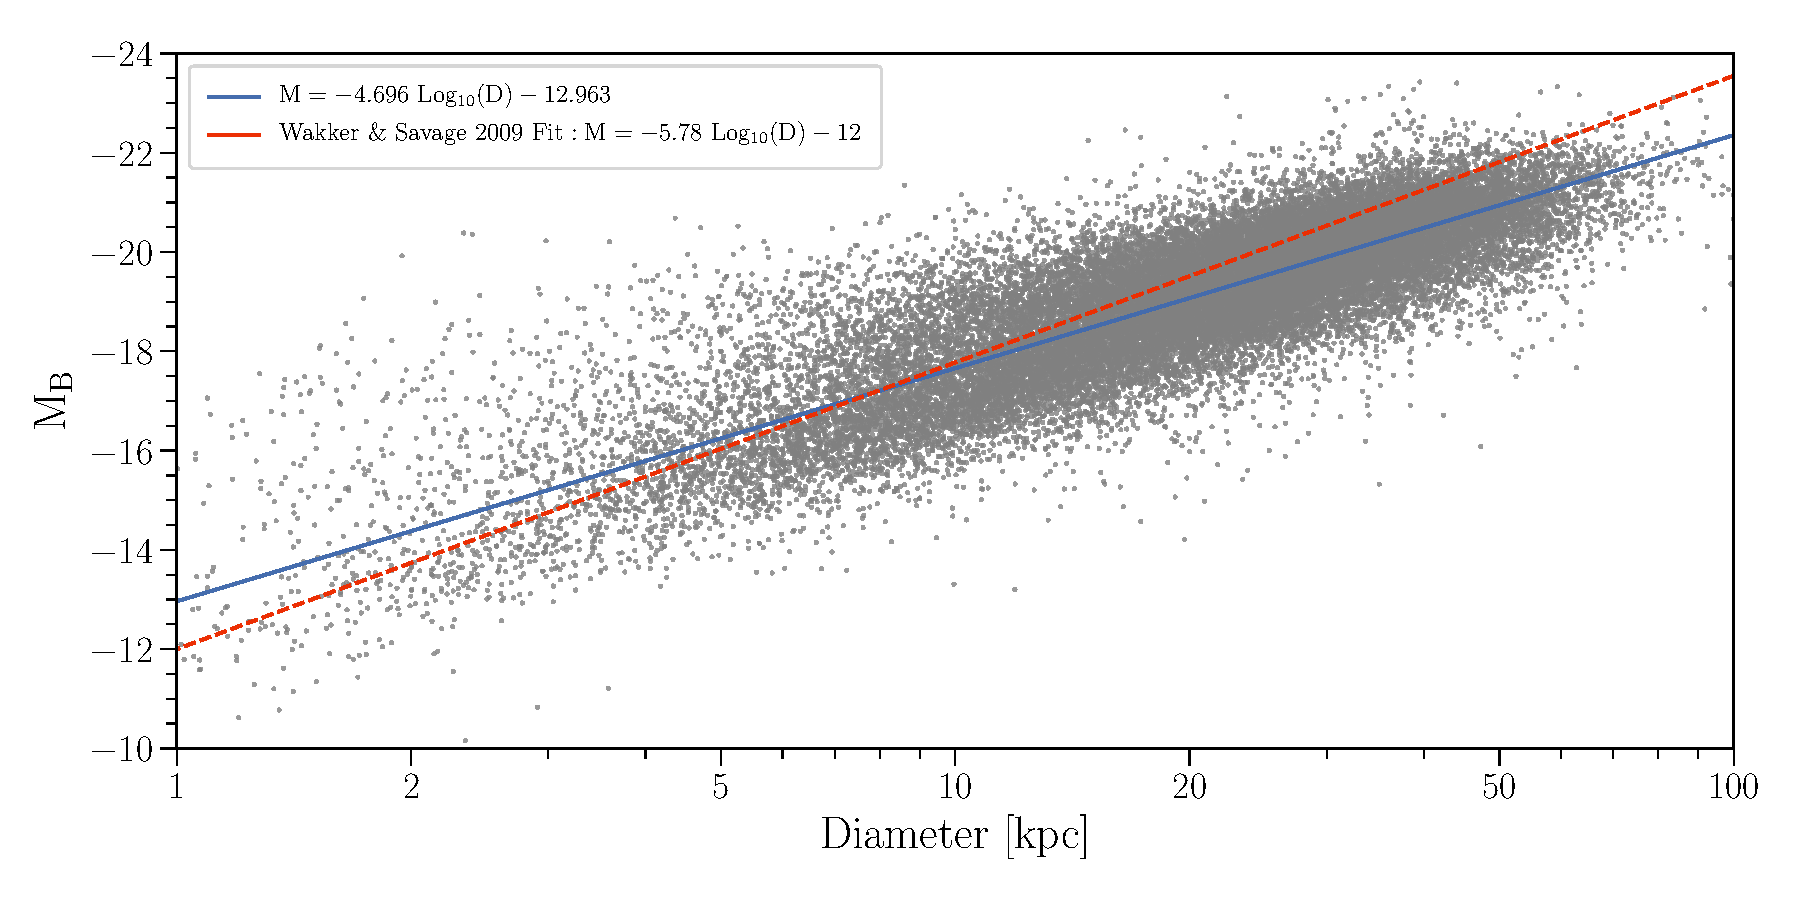
\includegraphics[width=0.99\textwidth]{Chap2/figures/mag_v_diam_fit2.pdf}
        \caption{\small{Relationship between absolute $B$-band magnitude and physical diameter for all galaxies with available data. Data are in grey, and a least-squares fit is shown in blue. The functional form of this fit is $M ~=~ a ~ log_{10}(D) + b$, with fit parameters $a = -4.696 \pm 0.01$ and $b = -12.963 \pm 0.01$. We also include the fit derived by \cite{wakker2009} in dashed-red.}}
%        \vspace{-5pt}
        \label{magvdiam}
\end{figure}


\subsection{MinDiam\_ang} \label{MinDiam_ang}
Minor axis diameter in units of arcsec. See \ref{diameters} for a complete discussion.

\subsection{e\_MajDiam\_ang} \label{e_MinDiam_ang}
Major axis diameter error. This error is purely a result of the $1\sigma$ fit error to K\_s (2MASS) values, and thus does not take into account any observational errors.

\subsection{e\_MinDiam\_ang} \label{e_MinDiam_ang}
Minor axis diameter error. This error is purely a result of the $1\sigma$ fit error to K\_s (2MASS) values, and thus does not take into account any observational errors.

\subsection{MajDiam} \label{MajDiam}
Linear major axis diameter in units of kpc, calculated using $bestDist$. See \ref{diameters} for a complete discussion.

\subsection{MinDiam} \label{MinDiam}
Linear minor axis diameter in units of kpc, calculated using $bestDist$. See \ref{diameters} for a complete discussion.

\subsection{e\_MajDiam} \label{e_MajDiam}
Linear major axis diameter error. This error is purely a result of the $1\sigma$ fit error to K\_s (2MASS) values, and thus does not take into account any observational errors.

\subsection{e\_MinDiam} \label{e_MinDiam}
Linear minor axis diameter error. This error is purely a result of the $1\sigma$ fit error to K\_s (2MASS) values, and thus does not take into account any observational errors.

\subsection{R\_vir} \label{R_vir}
Virial radius estimate calculated as

\begin{equation}
log R_{vir} = 0.69 log D + 1.24.
\end{equation}

\noindent This follows the parametrization of \cite{stocke2013} relating a galaxy's luminosity to its virial radius, combined with the \cite{wakker2009} empirical relation between diameter and luminosity (see \citealt{wakker2015} and references therein for further details).

\subsection{inc} \label{inc}
Galaxy inclination calculated simply as $inc = \cos^{-1} (MinDiam / MajDiam)$ in units of degrees.

\subsection{adjustedInc} \label{adjustedInc}
Galaxy inclination calculated assuming a finite disk thickness following \cite{heidmann1972}:

\begin{equation}
	\cos(i) = \sqrt{\frac{q^2 - q_0^2}{1 - q_0^2}},
	\label{incEq}
\end{equation}

\noindent where $q$ is the ratio of minor to major axes and $q_0$ is the minimum disk thickness. We set $q_0 = 0.2$ for all galaxies. This value is a compromise, as some galaxies (e.g., Sc type) will have intrinsic $q_0$ closer to $\sim 0.13$, while highly bulged galaxies will have larger $q_0$ (e.g., see \citealt{heidmann1972c}). However, as morphologies are only available for a subset of galaxies, a generic inclination correction fits our need for homogeneity. The result is that very thin galaxies will be slightly biased towards higher inclination and vice-versa with thicker galaxies.

\subsection{e\_inc} \label{e_inc}
Inclination error derived from the error in major and minor axes fits (see \ref{diameters}). Measurement errors for diameters, axis-ratios, and position angles are inconsistently reported in NED, so this value only captures the additional error introduced by converting non-2MASS diameters. For consistency, we set 2MASS diameter errors uniformly at 5\%.

\subsection{PA} \label{PA}
Position angle in units of degrees. When multiple PA measurements are available for a given target, we choose the highest ranking measurement as outlined in \ref{diameters}.

\subsection{diam\_key} \label{diameter_key}
The chosen source of our diameter value. Published diameters are converted to an equivalent 2MASS $K_s$ ``total" value following the fits given in Table \ref{diameter_fits}.

\subsection{ratio\_key} \label{ratio_key}
The chosen source of our diameter axis-ratio value. This is used to calculate the minor axis diameters and inclinations (see Table \ref{diameter_fits}).

\subsection{pa\_key} \label{pa_key}
The chosen source of our position angle value (see Table \ref{diameter_fits}).

\subsection{RC3\_type} \label{RC3_type}
Galaxy morphology as published in the Third Reference Catalogue of Bright Galaxies (RC3; see Table 2 in Section 3.3.a, page 15, of the printed RC3; \citealt{RC3}). Galaxies not included in RC3 are marked `x'.

\subsection{RC3\_d25} \label{RC3_d25}
The RC3 apparent major isophotal diameter measured at the 25th magnitude surface-brightness level, in units of B-mag per arcsecond (see Section 3.4.a, page 21, of Volume I of the printed RC3; \citealt{RC3}).

\subsection{RC3\_r25} \label{RC3_r25}
The RC3 ratio of the major to minor axis isophotal diameter, converted from decimal logarithm to a straight ratio in order to match the units of $ratio\_key$ (see Section 3.4.b, page 26, of Volume I of the printed RC3; \citealt{RC3}).

\subsection{RC3\_pa} \label{RC3_pa}
The RC3 position angle in units of degrees (see Section 3.5.a, page 30, of Volume I of the printed RC3; \citealt{RC3}).

\subsection{group\_num} \label{group_num}
Group designation number taken from the \cite{tully2015} group catalogue.

\subsection{group\_mem} \label{group_mem}
Number of members in this galaxy group taken from the \cite{tully2015} group catalogue.

\subsection{group\_dist} \label{group_dist}
Distance to the galaxy group, taken from the \cite{tully2015} group catalogue.

\subsection{MType} \label{MType}
Morphological type as homogenized by NED. We have removed extraneous space characters, and then replaced the individual spaces with underscore characters.

\subsection{flag} \label{flag}
A flag to help identify suspected issues with a galaxy. For most objects $flag=0$. If, however, we suspect an object to be a star we set $flag=1$. Our criteria for this is as follows: 1) if an object has $Vhel < 500$ \kms, no diameter measurement, and no $MType$ available, 2) if $MType$ is found to match any of our exclude morphologies. Our full exclude list is the following: [`:', `0.9', `0.92', `14.247', `14.632', `14.728', `14.818', `14.998', `14', `15.159', `15.171', `15.242', `15.341', `15.458', `15.79', `15.819', `16.281', `16.309', `16.348', `16.394', `16.556', `16.736', `16.764', `16.783', `16.981', `16', `17.012', `17.039', `17.441', `17.597', `2\_compacts', `2\_or\_3?\_spirals', `2\_S0\_galaxies', `2\_S0\_pec\_galaxies', `2\_SB0?\_pec\_galaxies', `2\_Spec?', `2\_spirals', `2\_symm.sp.arms', `2E', `2MASS\_Extended\_Ver.2', `3\_S0\_galaxies', `A-star', `A', `A0', `A3\_HII', `AGN:', `AGN?', `AGN', `AGN+SF', `AGN1', `AGN2', `ALG', `Amorphous', `B...', `B', `bright\_near*', `Cand.\_glob.\_cluster', `Candidate\_AGN', `Candidate\_PN', `Carbon', `D', `DA-star', `DA:', `DA', `DA\_auto', `DA+M:;\_Cand.\_QSO', `DA+M:', `DA+M', `DANS?', `DANS?\_Sbrst', `DANS', `DANS\_WR?', `DBA', `DC:', `DGTO', `DISRPTD', `DISTRBD', `DQ;\_Cand.\_QSO', `DQ:', `DSa', `F', `F2', \\ `F6-F8;Candidate\_WD', `High\_vel.\_cloud', `K\_Star', `K1', `K4-K5;Candidate\_WD', `M', `M\_star', `M\_Star', `M0', `M0V', `M1', `M3-M4', `O', `Opt.var.', `Planetary, `Planetary?', `Planetary\_nebula', `PN:', `PN?', `Point\_Src\_[SDSS]', `Possible\_*Cl', `Possible\_star', `star:', `star??', `star?', `stellar-like', `stellar:', `stellar',\_or\_galaxy', `M-star']

%[`M-star', `M star', `Opt.var.', `K4-K5;Candidate WD', `F6-F8;Candidate WD', `A', `Candidate AGN', `M1', `star??', `O', `K Star', `PN?', `K1', `M0', `M0V', `A0', `DA-star', `High vel. cloud', `O', `Carbon', `Point Src [SDSS]', `Possible star', `Planetary nebula', `M3-M4', `F2', `A-star', `PN:', `Cand. glob. cluster', `Candidate PN', `F'].

Secondly, we set $flag = 2$ if the velocity implied by $RID\_median$ (i.e., $RID\_median$ * $H_{\rm 0}$) differs from $Vhel$ by more than 1500 \kms. If $flag = 2$, it may be wise to use $distvcorr$ instead of $bestDist$. There is no overlap between flag types, so no possible stars ($flag=1$) objects have a redshift-independent distance available.


\subsection{lumClass} \label{lumClass}
Luminosity class as assigned by NED. Roman numerals between I, II, III, IV, and V designate galaxies in order of decreasing luminosity in an analogous fashion to the standard stellar luminosity classes.

\subsection{E(B-V)} \label{E(B-V)}
Galactic mean dust extinction in the direction of each galaxy from \cite{schlafly2011}.\footnote{See \url{https://irsa.ipac.caltech.edu/applications/DUST/}}
%Schlafly and Finkbeiner (2011)


\subsection{Bmag} \label{Bmag}
The median $B$-band apparent magnitude. For each galaxy we retrieved all $B$-band and SDSS $g$, $r$, and $z$ measurements. Direct $B$-band measurements are available for $\sim 30\%$ of galaxies, and a large fraction of the remaining objects have SDSS magnitudes. We convert SDSS magnitudes to $B$-band via $B = g + 0.39 (g-r) + 0.21$ \citep{jester2005}. Per SDSS DR12 guidelines, we preferentially selected SDSS $petrosian$ magnitudes when available, followed by $model$ and $cmodel$ values if $petrosian$ was not available. We then selected the min, max and median $B$-band values when more than one was available for inclusion in the final data product. SDSS-converted $B$-band values are included as a separate estimate ($Bmag\_sdss$; \S \ref{Bmag_sdss}). 

\subsection{Bmag\_key} \label{Bmag_key}
The name of the source or catalog responsible for producing our chosen value of $Bmag$.

\subsection{Bmag\_max}
The brightest $B$-band magnitude available in NED for this object. See \ref{Bmag} for details.

\subsection{Bmag\_max\_key}
The name of the source or catalog responsible for producing $Bmag\_max$.

\subsection{Bmag\_min}
The dimmest $B$-band magnitude available in NED for this object. See \ref{Bmag} for details.

\subsection{Bmag\_min\_key}
The name of the source or catalog responsible for producing $Bmag\_min$.

\subsection{Bmag\_sdss} \label{Bmag_sdss}
SDSS $g$ and $r$-band measurements converted to $B$-band apparent magnitude via $B = g + 0.39 (g-r) + 0.21$ \citep{jester2005}. See \ref{Bmag} for details.

\subsection{gmag\_sdss}
SDSS $g$-band apparent magnitude. This value is used in the $Bmag\_sdss$ calculation (see \S \ref{Bmag}).

\subsection{rmag\_sdss}
SDSS $r$-band apparent magnitude. This value is used in the $Bmag\_sdss$ calculation (see \S \ref{Bmag}).

\subsection{zmag\_sdss}
SDSS $z$-band apparent magnitude (see \S \ref{Bmag}).

\subsection{Lstar\_med} \label{Lstar_med}
The $L / $\Lstar ratio calculated using $Bmag$ and $bestDist$. We compute luminosity in units of \Lstar for each of the min, median, max and SDSS $B$-band values as follows:

\begin{equation}
	\frac{L}{L^*} = 10^{-0.4 (M_{\rm B} - M_{\rm B^{*}})},
	\label{lstar}
\end{equation}

\noindent where $M_{\rm B}$ is the galaxy absolute magnitude, calculated using the $bestDist$ distance estimate as described above. We adopted the CfA galaxy luminosity function by \citep{marzke1994}, which sets $B^{*} $ = -19.57. 


\subsection{e\_Lstar\_med} \label{e_Lstar_med}
$Lstar\_med$ error calculated with $e\_Bmag$ and $e\_bestDist$. Combining these errors leads to the following error formula:

\begin{equation}
	e\_Lstar\_med = 0.921 \sqrt{10^{-0.8(M - M^*)}  \Delta m^2},
\end{equation}
\noindent where $\Delta m$ is the error in $Bmag$.

%Errors from $E(B-V)$ are relatively negligible and thus were not included.


\subsection{Lstar\_max}
The $L / $\Lstar  ratio calculated using $B\_max$ and $bestDist$ + $e\_bestDist$ following Eq. \ref{lstar}. \\


\subsection{e\_Lstar\_max}
$Lstar\_max$ error calculated with $e\_Bmag\_max$ and $e\_bestDist$ (see \S \ref{e_Lstar_med}).


\subsection{Lstar\_min}
The $L / $\Lstar ratio calculated using $B\_min$ and $bestDist$ - $e\_bestDist$ following Eq. \ref{lstar}.


\subsection{e\_Lstar\_min}
$Lstar\_min$ error calculated with $e\_Bmag\_min$ and $e\_bestDist$ (see \S \ref{e_Lstar_med}).


\subsection{Lstar\_sdss}
The $L / $\Lstar ratio calculated using $Bmag\_sdss$ and $bestDist$ following Eq. \ref{lstar}.


\subsection{e\_Lstar\_sdss}
$Lstar\_sdss$ error calculated with $e\_bestDist$ and \cite{jester2005} conversion errors (see \S \ref{e_Lstar_med}).


\subsection{altNames}
The NED list of alternative object names for this galaxy with spaces removed. In the main catalogue we have included only NGC, IC, UGC, SDSS, and 2MASS names in this column. The associated alternative names catalogue contains the full list. Note that our preferred name, $Name$, and $NEDname$ will only appear in the $altNames$ list if they match these same criteria.\\


\section{Limitations \& Future}
This catalogue represents a significant step toward homogenization of the existing galaxy data within the $cz \leq 10,000$ \kms~redshift range. However, the resulting catalogue is not meant to be entirely robust or comprehensive - rather its purpose is to present a common batch of parameters for nearby galaxies in a easily retrievable and machine-readable manner. We have nonetheless endeavored to provide reasonable error estimates on all derived quantities and for as many observed quantities as possible.

Some caveats:

\begin{enumerate}

\item{This is not the result of a targeted survey or observing program, so its coverage and completeness is inherently non-uniform. We have endeavored to quantify this non-uniformity in Section \ref{completeness}. A future version of this catalogue will include all-sky coverage maps for each relevant major input catalog (e.g., SDSS, 2MASS, etc.).}

\item{The quality of the data and observational errors are difficult to determine. Hence, we present this dataset as more of a convenient "quick-look" directory than a scientifically rigorous data product.}

\item{This catalogue will soon be made available online as a searchable SQL database, and downloadable in csv and ascii-fixed-width formats.}
\end{enumerate}


\acknowledgements

This research has made use of the NASA/IPAC Extragalactic Database (NED) which is operated by the Jet Propulsion Laboratory, California Institute of Technology, under contract with the National Aeronautics and Space Administration. 

%Based on observations with the NASA/ESA \textit{Hubble Space Telescope}, obtained at the Space Telescope Institute, which is operated by AURA, Inc., under NASA contract NAS 5-26555.

%\nocite{*}
\bibliographystyle{thesis}
%\bibliography{/Users/clairemurray/Desktop/DMF_thesis/bib}
\bibliography{/Users/frenchd/Research/inclination/git_inclination/thesis/DMF_thesis/bib}




